% ============================================================
%  \section{API Designs Specification}
%  aBridgeAI — Capstone Report
%  Requires in preamble: longtable, graphicx, float, url (or hyperref),
%  booktabs, xcolor, tabularx, listings
%  NOTE: \path{} (from the url package) is used for API paths in tables
%  to allow automatic line breaking at '/' characters and prevent overflow.
% ============================================================

\section{API Designs Specification}
\label{appendix:api-design}

% ────────────────────────────────────────────────────────────
\subsection{Architecture \& Design Philosophy}
% ────────────────────────────────────────────────────────────

The aBridgeAI backend is a Python FastAPI service exposing a versioned RESTful API at the base path \path|/api/v1|. It serves as the single data contract between the Vite + TanStack Router single-page application and the server. The API surface is composed by a single \path|create_app()| factory that mounts every per-feature router under the shared \path|API_V1_PREFIX|; routers themselves carry their own per-feature prefix (e.g.\ \path|/teacher|, \path|/me/notifications|, \path|/admin/processing|). The platform follows six guiding principles:

\begin{enumerate}
    \item \textbf{Vertical-slice feature layout} --- each feature owns a self-contained directory under \path|abridgeai/features/<feature>/| with its own \path|routers/|, \path|services/|, \path|queries/|, and \path|schemas/| sub-packages. Routers translate HTTP to application calls; they never touch persistence directly. An import-linter contract (\textit{``Routers do not call queries directly''}) enforces the boundary at CI time.

    \item \textbf{Audience-scoped routers} --- a feature exposes one router per audience. The most common split is \path|learner| (the calling student, scoped under \path|/me/...|) versus \path|authoring| (instructor write operations, under \path|/teacher/...|), with optional \path|administration| (under \path|/admin/...|), \path|assignment| (department-level, under \path|/dept/...|) and \path|management| (educational-manager, under \path|/management/...|) routers. The URL prefix communicates the access context at a glance.

    \item \textbf{Bearer-token authentication via JWT} --- the API uses OAuth-only authentication (Google SSO). On a successful Google callback, the server returns a JSON body containing an \path|access_token| and a \path|refresh_token|; the SPA stores them and presents the access token as an \path|Authorization: Bearer <token>| header on every authenticated request. There is no traditional username/password endpoint and no CSRF middleware --- the bearer scheme on a header is not vulnerable to cross-site form submission.

    \item \textbf{MFA gate as a dependency} --- when a user has TOTP enabled, the access token is initially issued with a \textit{pre-MFA} marker. A FastAPI dependency on every protected endpoint refuses traffic until the holder of the token completes \path|POST /auth/me/mfa/challenge| followed by \path|POST /auth/me/mfa/verify|; the dependency rejects with HTTP 403 and a stable \path|mfa_required| error code so the SPA can route to the MFA challenge screen.

    \item \textbf{JSON-first, snake\_case field naming} --- all request and response bodies use JSON with \path|snake_case| field names (Pydantic v2 schemas). IDs are UUID v4, timestamps are ISO~8601 UTC strings, and enumerations are lowercase or lowercase-with-hyphens. Numeric ranges (\path|min_length|, \path|max_length|, \path|ge|/\path|le|) are validated by Pydantic at the FastAPI boundary, returning a 422 with a structured \path|detail| array.

    \item \textbf{Async-first request handling} --- every router function is \path|async def|, every database session is an \path|AsyncSession| from SQLAlchemy 2.0 async, and long-running AI work (quiz generation, interview question regeneration, material reprocessing) is dispatched to an ARQ worker pool over Redis rather than executed in-request. The HTTP layer therefore returns within hundreds of milliseconds even for AI-driven mutations; the SPA polls a \path|generation-runs/{run_id}| endpoint to surface progress.
\end{enumerate}

The backend deploys behind an HTTPS-terminating reverse proxy and emits security headers (HSTS, CSP, X-Frame-Options, X-Content-Type-Options, Referrer-Policy) via a dedicated \path|SecurityHeadersMiddleware|. Every HTTP request is recorded by an \path|AuditLogMiddleware| into the \path|http_audit_log| table with method, path, status, actor, and request ID, providing a per-request trace for security and performance debugging.

% ────────────────────────────────────────────────────────────
\subsection{Authentication Strategy}
% ────────────────────────────────────────────────────────────

The platform offers a single sign-in path: Google SSO. Username/password, password-reset, and email-verification endpoints intentionally do not exist --- this eliminates an entire class of credential-related bugs and shifts identity-proofing to Google's hardened identity provider.

\paragraph{Token Pair.} The application issues an access/refresh token pair as the canonical authentication primitive. The \textbf{access token} is a stateless HS256-signed JWT carrying \path|sub| (user ID), \path|sid| (session ID), \path|iat|, and \path|exp|. It is the only credential validated on every API request; the JWT decode is performed in memory and the embedded \path|sid| is then resolved against \path|auth_sessions| (with a Redis hot-path cache) to detect revocation and MFA gate state. The \textbf{refresh token} is a high-entropy opaque random string (URL-safe, 32 bytes) returned to the client once on login; the server persists only its SHA-256 hash in \path|auth_sessions.refresh_token_hash|, never the raw value. The access token has a 15-minute lifetime; the refresh token has a 7-day lifetime tied to the session row's \path|expires_at|. Refresh rotates both tokens (a new random refresh value, a new JWT) on every call.

\begin{longtable}{|p{0.16\textwidth}|p{0.27\textwidth}|p{0.12\textwidth}|p{0.32\textwidth}|}
    \caption{Token Pair --- backend storage} \label{tab:auth_tokens} \\
    \hline
    \textbf{Token} & \textbf{Purpose} & \textbf{Lifetime} & \textbf{Backend storage} \\
    \hline
    \endfirsthead
    \multicolumn{4}{c}{\small\tablename~\thetable{} \textit{(continued)}} \\
    \hline
    \textbf{Token} & \textbf{Purpose} & \textbf{Lifetime} & \textbf{Backend storage} \\
    \hline
    \endhead
    \hline
    \endfoot
    \path|access_token| & Authenticates every API request via \path|Authorization: Bearer| & 15 minutes & Stateless JWT, never persisted on the server; \path|sid| claim resolved against \path|auth_sessions| on each request. \\
    \hline
    \path|refresh_token| & Rotates the access/refresh pair via \path|POST /auth/refresh| & 7 days & Raw value returned to client once; only SHA-256 hash stored in \path|auth_sessions.refresh_token_hash| (\path|UNIQUE NOT NULL|). Rotated on every refresh. \\
    \hline
\end{longtable}

\paragraph{Hot-path session cache.} On every authenticated request the backend must verify that the JWT's \path|sid| still references a live, non-revoked, MFA-cleared session. To keep this check off PostgreSQL the session state is cached in Redis under \path|session:{session_id}| with a 60-second TTL --- short enough that an admin-triggered revoke (which also invalidates the cache) takes effect within seconds even if pub/sub invalidation fails. A reverse-index Redis \path|SET| at \path|user_sessions:{user_id}| stores the active session IDs for a user, enabling \path{O(N)} cascade revocation when an administrator disables an account without an unsafe \path|SCAN MATCH session:*|. The cache is read-through with safe fallback: any \path|RedisError| or connection failure logs a warning and the request transparently falls through to the source database, so a Redis outage degrades latency rather than availability.

\paragraph{Login Flow.}
\begin{enumerate}
    \item \path|GET /auth/google/login| returns \path|{authorization_url, state}|; the SPA stores \path|state| and redirects the browser to \path|authorization_url|.
    \item Google redirects back to \path|/auth/google/callback?code=...&state=...|. The SPA verifies the \path|state| matches and forwards the \path|code| to the backend.
    \item \path|GET /auth/google/callback| exchanges the code with Google, finds or rejects the application user (the platform requires the email to match a pre-provisioned account --- self-signup is not supported), and returns \path|{access_token, refresh_token, expires_in, requires_mfa, user}|.
    \item If \path|requires_mfa| is \path|true| the SPA navigates to the MFA challenge screen and calls \path|POST /auth/me/mfa/challenge| then \path|POST /auth/me/mfa/verify|. On successful verification the backend re-issues a token pair flagged as MFA-completed.
\end{enumerate}

\paragraph{Refresh Flow.} The SPA submits the current refresh token to \path|POST /auth/refresh|; the server validates the session row, rotates the refresh token, and returns a new pair. Token rotation is mandatory --- a refresh token cannot be reused twice.

\paragraph{Logout.} \path|POST /auth/logout| invalidates the refresh-token row server-side; the SPA discards the local pair. Subsequent requests that present the discarded pair receive HTTP 401.

% ────────────────────────────────────────────────────────────
\subsection{Multi-Factor Authentication}
% ────────────────────────────────────────────────────────────

TOTP-based MFA is exposed as a self-service feature under \path|/auth/me/mfa|. Enrollment is two-step: \path|POST .../totp/enroll| generates a TOTP secret and returns the \path|otpauth://| URL plus a transient \path|factor_id|; the user scans the QR in an authenticator app and confirms with \path|POST .../totp/verify| supplying the first generated code. Successful verification produces a one-time set of recovery codes (\path|MfaRecoveryCodesResponse|) that the SPA must persist for the user.

Once enrolled, every fresh login produces a pre-MFA token. \path|POST .../challenge| returns a \path|challenge_id|; \path|POST .../verify| accepts either a 6--8 digit TOTP code or a single-use recovery code. Both \path|.../recovery-codes/regenerate| and \path|.../disable| require recent MFA verification --- they enforce the same code/recovery-code proof-of-possession check inline so a stolen access token cannot silently turn off the second factor.

\begin{longtable}{|p{0.1\textwidth}|p{0.371\textwidth}|p{0.409\textwidth}|}
    \caption{MFA endpoints} \label{tab:mfa_endpoints} \\
    \hline
    \textbf{Method} & \textbf{Path} & \textbf{Description} \\
    \hline
    \endfirsthead
    \multicolumn{3}{c}{\small\tablename~\thetable{} \textit{(continued)}} \\
    \hline
    \textbf{Method} & \textbf{Path} & \textbf{Description} \\
    \hline
    \endhead
    \hline
    \endfoot
    GET    & \path|/auth/me/mfa/status|              & Whether the caller has TOTP enrolled and the session's \path|mfa_verified_at|. \\
    \hline
    POST   & \path|/auth/me/mfa/totp/enroll|         & Provision a fresh TOTP secret and return the otpauth URL. \\
    \hline
    POST   & \path|/auth/me/mfa/totp/verify|         & Confirm enrollment with the first valid code; emit recovery codes. \\
    \hline
    POST   & \path|/auth/me/mfa/challenge|           & Open a challenge during a fresh login. \\
    \hline
    POST   & \path|/auth/me/mfa/verify|              & Verify a TOTP code or recovery code against the open challenge. \\
    \hline
    POST   & \path|/auth/me/mfa/recovery-codes/regenerate| & Wipe and re-issue recovery codes (requires inline proof). \\
    \hline
    POST   & \path|/auth/me/mfa/disable|             & Disable MFA; requires inline proof-of-possession. \\
    \hline
\end{longtable}

% ────────────────────────────────────────────────────────────
\subsection{Error Handling}
% ────────────────────────────────────────────────────────────

Errors surface as standard FastAPI \path|HTTPException| responses with a JSON body of \path|{detail: ...}| and a numeric status code. The application defines a small hierarchy of exceptions (\path|AppError|, \path|NotFoundError|, \path|UnauthorizedError|, \path|ForbiddenError|, \path|ConflictError|) raised by the service layer and translated to HTTP at the router boundary. For richer cases (OAuth provisioning, MFA gates, validation failures) the \path|detail| is an object that carries a stable \path|error| code so the SPA can branch deterministically:

\begin{verbatim}
HTTP/1.1 403 Forbidden
Content-Type: application/json

{
  "detail": {
    "error": "oauth_account_not_provisioned",
    "message": "This Google account is not linked to a registered user."
  }
}
\end{verbatim}

\begin{longtable}{|p{0.105\textwidth}|p{0.302\textwidth}|p{0.473\textwidth}|}
    \caption{Common HTTP status codes} \label{tab:status_codes} \\
    \hline
    \textbf{Code} & \textbf{Name} & \textbf{Used For} \\
    \hline
    \endfirsthead
    \multicolumn{3}{c}{\small\tablename~\thetable{} \textit{(continued)}} \\
    \hline
    \textbf{Code} & \textbf{Name} & \textbf{Used For} \\
    \hline
    \endhead
    \hline
    \endfoot
    200 & OK                    & Successful read or successful synchronous mutation. \\ \hline
    201 & Created               & Resource created; body returns the new resource. \\ \hline
    202 & Accepted              & AI generation accepted and queued (response carries a \path|run_id|). \\ \hline
    204 & No Content            & Successful mutation with no payload (e.g.\ delete). \\ \hline
    400 & Bad Request           & Domain-level validation failure raised as \path|AppError|. \\ \hline
    401 & Unauthorized          & Missing or invalid bearer token; carries \path|WWW-Authenticate: Bearer|. \\ \hline
    403 & Forbidden             & RBAC denial, MFA required, or account not provisioned. \\ \hline
    404 & Not Found             & \path|NotFoundError| --- entity does not exist or is invisible to caller. \\ \hline
    409 & Conflict              & \path|ConflictError| --- e.g.\ slug collision, optimistic-lock violation. \\ \hline
    422 & Unprocessable Entity  & Pydantic validation failure on the request body or query string. \\ \hline
    503 & Service Unavailable   & Upstream provider error (Google OAuth, AI provider, Redis). \\ \hline
\end{longtable}

% ────────────────────────────────────────────────────────────
\subsection{Pagination, Filtering and Idempotency}
% ────────────────────────────────────────────────────────────

\paragraph{Pagination.} Every list endpoint uses \textbf{cursor pagination}. The shared \path|core/pagination/cursor.py| module exposes a generic \path|CursorPage[T]| dataclass; all list responses are wrapped as \verb*~{items: T[], next_cursor: string | null}~. The cursor is opaque to the client --- typically a base64-encoded UUID of the last row returned, or an ISO-8601 \path|created_at| timestamp for time-ordered feeds (notifications, audit trails). Clients pass it back as \path|?cursor=...| (paired with an optional \path|limit|, default 20, max 100) to fetch the next page; \path|next_cursor| being \path|null| signals end-of-list. Cursor pagination keeps queries on a single index column, scales to deep traversal without the \path{O(N)} skip cost of \path|OFFSET|, and is not perturbed by inserts or deletes between page fetches --- the user never sees a duplicated or skipped row mid-scroll.

\paragraph{Filtering and sorting.} List endpoints accept feature-specific filters as query parameters (e.g.\ \path|status=published|, \path|role=teacher|, \path|q=<search>|). Sort order is fixed per endpoint and documented inline; freeform sort keys are deliberately not supported to keep the index strategy predictable.

\paragraph{Idempotency.} Mutating endpoints that may be retried by the SPA (in particular \path|POST .../attempts| during quiz submission and the bulk \path|POST .../quizzes/{id}/generate|) accept an optional \path|Idempotency-Key| header; the backend deduplicates against this key for a 24-hour window. AI generation endpoints additionally return an \path|Operation-Location| header pointing to \path|.../generation-runs/{run_id}| for progress polling.

% ────────────────────────────────────────────────────────────
\subsection{Endpoint Catalogue}
% ────────────────────────────────────────────────────────────

The following tables enumerate every endpoint exposed by the backend, grouped by feature and audience. All paths are relative to \path|/api/v1|. The \textit{Auth} column reads ``Bearer'' when an authenticated session is required (the default), ``Public'' for anonymous endpoints, and ``Bearer + role'' when an additional role check applies.

% ── Identity ────────────────────────────────────────────────
\subsubsection{Identity --- Authentication \& Profile}

\begin{longtable}{|p{0.105\textwidth}|p{0.388\textwidth}|p{0.11\textwidth}|p{0.277\textwidth}|}
    \caption{Identity endpoints (Google OAuth, refresh, logout, profile).} \label{tab:api_identity} \\
    \hline
    \textbf{Method} & \textbf{Path} & \textbf{Auth} & \textbf{Description} \\
    \hline
    \endfirsthead
    \multicolumn{4}{c}{\small\tablename~\thetable{} \textit{(continued)}} \\
    \hline
    \textbf{Method} & \textbf{Path} & \textbf{Auth} & \textbf{Description} \\
    \hline
    \endhead
    \hline
    \endfoot
    GET    & \path|/auth/google/login|    & Public   & Return the Google OAuth authorisation URL plus an opaque \path|state|. \\ \hline
    GET    & \path|/auth/google/callback| & Public   & Exchange the Google authorisation code for an access/refresh pair. \\ \hline
    POST   & \path|/auth/refresh|         & Public$^\ast$ & Rotate the refresh token; returns a fresh token pair. \\ \hline
    POST   & \path|/auth/logout|          & Bearer   & Invalidate the current refresh-token row server-side. \\ \hline
    GET    & \path|/users/me|             & Bearer   & Return the authenticated user's profile. \\ \hline
    PATCH  & \path|/users/me/profile|     & Bearer   & Update display name, avatar, locale, etc. \\ \hline
    GET    & \path|/users/me/permissions| & Bearer   & Return effective roles and permission flags. \\ \hline
    GET    & \path|/users|                & Bearer   & Search users by name or email (auto-complete; admin-scoped). \\ \hline
    GET    & \path|/users/{user_id}|      & Bearer   & Return a public profile by ID. \\ \hline
\end{longtable}

\noindent$^\ast$\textit{The refresh token itself is the credential; no Bearer header is required.}

% ── Access control ──────────────────────────────────────────
\subsubsection{Access Control --- Roles, Grants \& Organisations}

\begin{longtable}{|p{0.105\textwidth}|p{0.425\textwidth}|p{0.11\textwidth}|p{0.24\textwidth}|}
    \caption{Access-control endpoints (admin-scoped).} \label{tab:api_access_control} \\
    \hline
    \textbf{Method} & \textbf{Path} & \textbf{Auth} & \textbf{Description} \\
    \hline
    \endfirsthead
    \multicolumn{4}{c}{\small\tablename~\thetable{} \textit{(continued)}} \\
    \hline
    \textbf{Method} & \textbf{Path} & \textbf{Auth} & \textbf{Description} \\
    \hline
    \endhead
    \hline
    \endfoot
    GET    & \path|/admin/permissions| & Bearer + admin & List the permission catalogue. \\ \hline
    GET    & \path|/admin/roles|       & Bearer + admin & List system and tenant roles with their permissions. \\ \hline
    GET    & \path|/admin/users/{user_id}/assignments|                          & Bearer + admin & List role assignments for a user. \\ \hline
    POST   & \path|/admin/users/{user_id}/assignments|                          & Bearer + admin & Assign a role to a user (optionally org-scoped). \\ \hline
    DELETE & \path|/admin/users/{user_id}/assignments/{assignment_id}|          & Bearer + admin & Revoke a role assignment. \\ \hline
    GET    & \path|/admin/users/{user_id}/grants|                               & Bearer + admin & List ad-hoc permission grants for a user. \\ \hline
    POST   & \path|/admin/users/{user_id}/grants|                               & Bearer + admin & Issue an ad-hoc permission grant. \\ \hline
    DELETE & \path|/admin/users/{user_id}/grants/{grant_id}|                    & Bearer + admin & Revoke an ad-hoc grant. \\ \hline
    GET    & \path|/admin/organizations|                                        & Bearer + admin & List tenant organisations. \\ \hline
    POST   & \path|/admin/organizations|                                        & Bearer + admin & Create a tenant organisation. \\ \hline
    GET    & \path|/admin/organizations/{org_id}|                               & Bearer + admin & Get an organisation. \\ \hline
    PATCH  & \path|/admin/organizations/{org_id}|                               & Bearer + admin & Update organisation settings. \\ \hline
    DELETE & \path|/admin/organizations/{org_id}|                               & Bearer + admin & Soft-delete an organisation. \\ \hline
    GET    & \path|/admin/organizations/{org_id}/domains|                       & Bearer + admin & List email domains owned by the organisation. \\ \hline
    POST   & \path|/admin/organizations/{org_id}/domains|                       & Bearer + admin & Add an owned email domain. \\ \hline
    PATCH  & \path|/admin/organization-domains/{domain_id}|                     & Bearer + admin & Update a domain (rename, mark verified). \\ \hline
    DELETE & \path|/admin/organization-domains/{domain_id}|                     & Bearer + admin & Remove an owned domain. \\ \hline
    GET    & \path|/admin/organizations/{org_id}/units|                         & Bearer + admin & List org units (faculties, departments). \\ \hline
    POST   & \path|/admin/organizations/{org_id}/units|                         & Bearer + admin & Create an org unit. \\ \hline
    GET    & \path|/admin/org-units/{unit_id}|                                  & Bearer + admin & Get an org unit. \\ \hline
    PATCH  & \path|/admin/org-units/{unit_id}|                                  & Bearer + admin & Update an org unit. \\ \hline
    DELETE & \path|/admin/org-units/{unit_id}|                                  & Bearer + admin & Delete an org unit. \\ \hline
    GET    & \path|/admin/organizations/{org_id}/memberships|                   & Bearer + admin & List user memberships in an organisation. \\ \hline
    POST   & \path|/admin/organizations/{org_id}/memberships|                   & Bearer + admin & Add a user to an organisation. \\ \hline
    PATCH  & \path|/admin/organization-memberships/{membership_id}|             & Bearer + admin & Update membership status. \\ \hline
    DELETE & \path|/admin/organization-memberships/{membership_id}|             & Bearer + admin & Remove a membership. \\ \hline
\end{longtable}

% ── Courses (learner) ───────────────────────────────────────
\subsubsection{Courses --- Learner}

\begin{longtable}{|p{0.105\textwidth}|p{0.425\textwidth}|p{0.11\textwidth}|p{0.24\textwidth}|}
    \caption{Course-learner endpoints (the calling user's own enrolments).} \label{tab:api_courses_learner} \\
    \hline
    \textbf{Method} & \textbf{Path} & \textbf{Auth} & \textbf{Description} \\
    \hline
    \endfirsthead
    \multicolumn{4}{c}{\small\tablename~\thetable{} \textit{(continued)}} \\
    \hline
    \textbf{Method} & \textbf{Path} & \textbf{Auth} & \textbf{Description} \\
    \hline
    \endhead
    \hline
    \endfoot
    GET    & \path|/me/courses/courses|                                                & Bearer & List the caller's enrolled courses. \\ \hline
    GET    & \path|/me/courses/courses/by-slug/{slug}|                                  & Bearer & Resolve a course by its public slug. \\ \hline
    GET    & \path|/me/courses/courses/{course_id}|                                     & Bearer & Get course detail. \\ \hline
    GET    & \path|/me/courses/courses/{course_id}/content|                             & Bearer & Get the full module/lesson tree. \\ \hline
    GET    & \path|/me/courses/courses/{course_id}/tags|                                & Bearer & Get the course's tags. \\ \hline
    GET    & \path|/me/courses/courses/{course_id}/outcomes|                            & Bearer & Get the course's learning outcomes. \\ \hline
    GET    & \path|/me/courses/courses/{course_id}/modules|                             & Bearer & List modules with publish state. \\ \hline
    GET    & \path|/me/courses/modules/{module_id}|                                     & Bearer & Get a module. \\ \hline
    GET    & \path|/me/courses/modules/{module_id}/items|                               & Bearer & List ordered lesson/quiz items. \\ \hline
    GET    & \path|/me/courses/modules/{module_id}/lessons|                             & Bearer & List lessons in a module. \\ \hline
    GET    & \path|/me/courses/lessons/{lesson_id}|                                     & Bearer & Get a lesson. \\ \hline
    GET    & \path|/me/courses/lessons/{lesson_id}/resources|                           & Bearer & List downloadable lesson resources. \\ \hline
    GET    & \path|/me/courses/lesson-resources/{resource_id}/download-url|             & Bearer & Issue a presigned S3 URL for a resource. \\ \hline
\end{longtable}

% ── Courses (authoring / dept / admin) ──────────────────────
\subsubsection{Courses --- Authoring (Teacher)}

\begin{longtable}{|p{0.1\textwidth}|p{0.424\textwidth}|p{0.15\textwidth}|p{0.206\textwidth}|}
    \caption{Course-authoring endpoints (teacher role).} \label{tab:api_courses_authoring} \\
    \hline
    \textbf{Method} & \textbf{Path} & \textbf{Auth} & \textbf{Description} \\
    \hline
    \endfirsthead
    \multicolumn{4}{c}{\small\tablename~\thetable{} \textit{(continued)}} \\
    \hline
    \textbf{Method} & \textbf{Path} & \textbf{Auth} & \textbf{Description} \\
    \hline
    \endhead
    \hline
    \endfoot
    POST   & \path|/teacher/courses|                                            & Bearer + teacher & Create a course. \\ \hline
    GET    & \path|/teacher/courses/check-slug|                                 & Bearer + teacher & Probe slug availability. \\ \hline
    GET    & \path|/teacher/courses|                                            & Bearer + teacher & List courses owned or co-taught by the caller. \\ \hline
    GET    & \path|/teacher/courses/{course_id}|                                & Bearer + teacher & Get a course (authoring view). \\ \hline
    GET    & \path|/teacher/courses/{course_id}/content|                        & Bearer + teacher & Get the full module/lesson/quiz tree. \\ \hline
    GET    & \path|/teacher/courses/{course_id}/roster|                         & Bearer + teacher & List enrolled students. \\ \hline
    PATCH  & \path|/teacher/courses/{course_id}|                                & Bearer + teacher & Update course metadata. \\ \hline
    POST   & \path|/teacher/courses/{course_id}/publish|                        & Bearer + teacher & Publish the course. \\ \hline
    POST   & \path|/teacher/courses/{course_id}/archive|                        & Bearer + teacher & Archive the course. \\ \hline
    POST   & \path|/teacher/courses/{course_id}/modules|                        & Bearer + teacher & Add a module. \\ \hline
    PATCH  & \path|/teacher/modules/{module_id}|                                & Bearer + teacher & Update a module. \\ \hline
    PUT    & \path|/teacher/modules/{module_id}/prerequisites|                  & Bearer + teacher & Set module prerequisites. \\ \hline
    PUT    & \path|/teacher/modules/{module_id}/items/reorder|                  & Bearer + teacher & Reorder module items (drag-and-drop). \\ \hline
    PATCH  & \path|/teacher/module-items/{module_item_id}|                      & Bearer + teacher & Update a module-item entry. \\ \hline
    DELETE & \path|/teacher/module-items/{module_item_id}|                      & Bearer + teacher & Remove a module-item entry. \\ \hline
    GET    & \path|/teacher/modules/{module_id}/lessons|                        & Bearer + teacher & List lessons within a module. \\ \hline
    POST   & \path|/teacher/modules/{module_id}/lessons|                        & Bearer + teacher & Create a lesson. \\ \hline
    GET    & \path|/teacher/lessons/{lesson_id}|                                & Bearer + teacher & Get a lesson. \\ \hline
    GET    & \path|/teacher/lessons/{lesson_id}/outline|                        & Bearer + teacher & Get the structural outline of the lesson. \\ \hline
    GET    & \path|/teacher/lessons/{lesson_id}/resources|                      & Bearer + teacher & List downloadable resources. \\ \hline
    PATCH  & \path|/teacher/lessons/{lesson_id}|                                & Bearer + teacher & Update a lesson. \\ \hline
    POST   & \path|/teacher/lessons/{lesson_id}/resources|                      & Bearer + teacher & Attach a resource. \\ \hline
    DELETE & \path|/teacher/lesson-resources/{resource_id}|                     & Bearer + teacher & Detach a resource. \\ \hline
    GET    & \path|/teacher/lesson-resources/{resource_id}/download-url|        & Bearer + teacher & Issue a presigned download URL. \\ \hline
\end{longtable}

\subsubsection{Courses --- Department \& Administration}

\begin{longtable}{|p{0.1\textwidth}|p{0.424\textwidth}|p{0.15\textwidth}|p{0.206\textwidth}|}
    \caption{Course department-assignment and administration endpoints.} \label{tab:api_courses_dept_admin} \\
    \hline
    \textbf{Method} & \textbf{Path} & \textbf{Auth} & \textbf{Description} \\
    \hline
    \endfirsthead
    \multicolumn{4}{c}{\small\tablename~\thetable{} \textit{(continued)}} \\
    \hline
    \textbf{Method} & \textbf{Path} & \textbf{Auth} & \textbf{Description} \\
    \hline
    \endhead
    \hline
    \endfoot
    GET    & \path|/dept/courses|                                       & Bearer + dept   & List courses for the caller's department. \\ \hline
    GET    & \path|/dept/courses/{course_id}/teachers|                  & Bearer + dept   & List teachers assigned to a course. \\ \hline
    POST   & \path|/dept/courses/{course_id}/teachers|                  & Bearer + dept   & Assign a teacher to a course. \\ \hline
    DELETE & \path|/dept/courses/{course_id}/teachers/{user_id}|        & Bearer + dept   & Unassign a teacher. \\ \hline
    GET    & \path|/dept/courses/{course_id}/roster|                    & Bearer + dept   & Read the enrolled-student roster. \\ \hline
    GET    & \path|/dept/org-units/{org_unit_id}/courses|               & Bearer + dept   & List courses owned by an org unit. \\ \hline
    GET    & \path|/admin/courses|                                      & Bearer + admin  & Cross-organisation course listing. \\ \hline
    POST   & \path|/admin/courses/{course_id}/restore|                  & Bearer + admin  & Restore a soft-deleted course. \\ \hline
    GET    & \path|/admin/courses/{course_id}/audit|                    & Bearer + admin  & Course-level audit trail. \\ \hline
    GET    & \path|/admin/courses/{course_id}/processing|               & Bearer + admin  & Per-course AI processing history. \\ \hline
    GET    & \path|/admin/courses/_stats|                               & Bearer + admin  & Cross-org course aggregates. \\ \hline
\end{longtable}

% ── Materials ───────────────────────────────────────────────
\subsubsection{Materials}

Material upload uses a two-phase protocol so large files can be streamed directly from the browser to the object store (Garage S3-compatible) without traversing the application server. The teacher first calls \path|init-upload| to receive a presigned URL or a multipart upload ID; the SPA then uploads the bytes; finally it calls \path|complete| (or \path|.../multipart/complete|) to register the version and trigger AI processing.

\begin{longtable}{|p{0.1\textwidth}|p{0.461\textwidth}|p{0.15\textwidth}|p{0.169\textwidth}|}
    \caption{Materials endpoints.} \label{tab:api_materials} \\
    \hline
    \textbf{Method} & \textbf{Path} & \textbf{Auth} & \textbf{Description} \\
    \hline
    \endfirsthead
    \multicolumn{4}{c}{\small\tablename~\thetable{} \textit{(continued)}} \\
    \hline
    \textbf{Method} & \textbf{Path} & \textbf{Auth} & \textbf{Description} \\
    \hline
    \endhead
    \hline
    \endfoot
    POST   & \path|/teacher/lessons/{lesson_id}/materials/init-upload|                                 & Bearer + teacher & Begin an upload (single-part or multipart). \\ \hline
    POST   & \path|/teacher/materials/{material_id}/versions/{version_id}/multipart/parts|             & Bearer + teacher & Issue per-part presigned URLs. \\ \hline
    POST   & \path|/teacher/materials/{material_id}/versions/{version_id}/multipart/complete|          & Bearer + teacher & Finalise a multipart upload. \\ \hline
    POST   & \path|/teacher/materials/{material_id}/versions/{version_id}/multipart/abort|             & Bearer + teacher & Abort a multipart upload. \\ \hline
    POST   & \path|/teacher/materials/{material_id}/versions/{version_id}/complete|                    & Bearer + teacher & Finalise a single-part upload and queue processing. \\ \hline
    GET    & \path|/teacher/lessons/{lesson_id}/materials|                                             & Bearer + teacher & List materials attached to a lesson. \\ \hline
    POST   & \path|/teacher/lessons/{lesson_id}/materials/link|                                        & Bearer + teacher & Link an existing material into another lesson. \\ \hline
    GET    & \path|/teacher/lessons/{lesson_id}/processing-summary|                                    & Bearer + teacher & Aggregate AI-processing state for a lesson. \\ \hline
    GET    & \path|/teacher/materials/{material_id}|                                                   & Bearer + teacher & Get material detail. \\ \hline
    GET    & \path|/teacher/materials/{material_id}/processing-summary|                                & Bearer + teacher & Per-material processing state. \\ \hline
    GET    & \path|/teacher/materials/{material_id}/stream-url|                                        & Bearer + teacher & Issue a presigned streaming URL (PDF/video). \\ \hline
    PATCH  & \path|/teacher/materials/{material_id}|                                                   & Bearer + teacher & Update material metadata. \\ \hline
    POST   & \path|/teacher/materials/{material_id}/reprocess|                                         & Bearer + teacher & Re-run AI ingestion on the latest version. \\ \hline
    DELETE & \path|/teacher/materials/{material_id}|                                                   & Bearer + teacher & Soft-delete a material. \\ \hline
    GET    & \path|/materials/{material_id}|                                                           & Bearer & Learner-facing material descriptor. \\ \hline
    GET    & \path|/materials/{material_id}/stream-url|                                                & Bearer & Learner-facing presigned streaming URL. \\ \hline
    GET    & \path|/materials/{material_id}/chunks/preview|                                            & Bearer & Preview the first N text chunks for review. \\ \hline
\end{longtable}

% ── Quizzes ─────────────────────────────────────────────────
\subsubsection{Quizzes}

Quiz authoring follows a draft / generate / review / publish pipeline. \path|POST .../quizzes/{quiz_id}/generate| accepts a generation spec (source lessons, count, mode, types) and returns a \path|run_id| immediately; the SPA polls \path|.../generation-runs/{run_id}| to surface progress. Generated questions land in a \textit{Pending Review} state and are visible to students only after explicit instructor approval.

\begin{longtable}{|p{0.1\textwidth}|p{0.461\textwidth}|p{0.15\textwidth}|p{0.169\textwidth}|}
    \caption{Quizzes endpoints.} \label{tab:api_quizzes} \\
    \hline
    \textbf{Method} & \textbf{Path} & \textbf{Auth} & \textbf{Description} \\
    \hline
    \endfirsthead
    \multicolumn{4}{c}{\small\tablename~\thetable{} \textit{(continued)}} \\
    \hline
    \textbf{Method} & \textbf{Path} & \textbf{Auth} & \textbf{Description} \\
    \hline
    \endhead
    \hline
    \endfoot
    POST   & \path|/teacher/courses/{course_id}/quizzes|                                       & Bearer + teacher & Create a quiz on a module. \\ \hline
    GET    & \path|/teacher/quizzes/{quiz_id}|                                                  & Bearer + teacher & Get authoring view of a quiz. \\ \hline
    PATCH  & \path|/teacher/quizzes/{quiz_id}|                                                  & Bearer + teacher & Update quiz metadata. \\ \hline
    POST   & \path|/teacher/quizzes/{quiz_id}/publish|                                          & Bearer + teacher & Publish the quiz. \\ \hline
    POST   & \path|/teacher/quizzes/{quiz_id}/questions/bulk-set-expected-time|                 & Bearer + teacher & Apply a uniform per-question time. \\ \hline
    DELETE & \path|/teacher/quizzes/{quiz_id}|                                                  & Bearer + teacher & Delete a quiz. \\ \hline
    POST   & \path|/teacher/quizzes/{quiz_id}/generate|                                         & Bearer + teacher & Queue an AI generation run; returns \path|run_id|. \\ \hline
    GET    & \path|/teacher/quizzes/{quiz_id}/generation-runs/latest|                           & Bearer + teacher & Latest generation-run status. \\ \hline
    GET    & \path|/teacher/quizzes/{quiz_id}/generation-runs/{run_id}|                         & Bearer + teacher & Specific run status. \\ \hline
    POST   & \path|/teacher/quizzes/{quiz_id}/questions|                                        & Bearer + teacher & Add a question manually. \\ \hline
    PATCH  & \path|/teacher/quizzes/{quiz_id}/questions/{question_id}|                          & Bearer + teacher & Update or approve a question. \\ \hline
    DELETE & \path|/teacher/quizzes/{quiz_id}/questions/{question_id}|                          & Bearer + teacher & Delete a question. \\ \hline
    POST   & \path|/teacher/quizzes/{quiz_id}/questions/{question_id}/regenerate|               & Bearer + teacher & Regenerate a single AI question. \\ \hline
    GET    & \path|/teacher/courses/{course_id}/question-bank|                                  & Bearer + teacher & Browse the course-level question bank. \\ \hline
    POST   & \path|/teacher/quizzes/{quiz_id}/questions/import|                                 & Bearer + teacher & Import from the question bank. \\ \hline
    GET    & \path|/quizzes/{quiz_id}|                                                          & Bearer & Learner view (questions only, no answers). \\ \hline
    POST   & \path|/quizzes/{quiz_id}/attempts|                                                 & Bearer & Start a new attempt. \\ \hline
    POST   & \path|/attempts/{attempt_id}/answers|                                              & Bearer & Submit one or more answers. \\ \hline
    POST   & \path|/attempts/{attempt_id}/submit|                                               & Bearer & Finalise the attempt; trigger scoring. \\ \hline
    GET    & \path|/attempts/{attempt_id}|                                                      & Bearer & Attempt detail. \\ \hline
    GET    & \path|/attempts/{attempt_id}/review|                                               & Bearer & Per-question review with correct answers. \\ \hline
    GET    & \path|/me/quizzes/{quiz_id}/attempts|                                              & Bearer & Caller's attempt history for the quiz. \\ \hline
\end{longtable}

% ── Interviews ──────────────────────────────────────────────
\subsubsection{Interviews}

\begin{longtable}{|p{0.1\textwidth}|p{0.461\textwidth}|p{0.15\textwidth}|p{0.169\textwidth}|}
    \caption{Interview endpoints (AI mock-interview surface).} \label{tab:api_interviews} \\
    \hline
    \textbf{Method} & \textbf{Path} & \textbf{Auth} & \textbf{Description} \\
    \hline
    \endfirsthead
    \multicolumn{4}{c}{\small\tablename~\thetable{} \textit{(continued)}} \\
    \hline
    \textbf{Method} & \textbf{Path} & \textbf{Auth} & \textbf{Description} \\
    \hline
    \endhead
    \hline
    \endfoot
    POST   & \path|/teacher/courses/{course_id}/interview-configs|                                & Bearer + teacher & Create an interview configuration. \\ \hline
    GET    & \path|/teacher/interview-configs/{config_id}|                                          & Bearer + teacher & Get a configuration. \\ \hline
    PATCH  & \path|/teacher/interview-configs/{config_id}|                                          & Bearer + teacher & Update a configuration. \\ \hline
    POST   & \path|/teacher/interview-configs/{config_id}/publish|                                  & Bearer + teacher & Publish the configuration. \\ \hline
    DELETE & \path|/teacher/interview-configs/{config_id}|                                          & Bearer + teacher & Delete a configuration. \\ \hline
    POST   & \path|/teacher/interview-configs/{config_id}/generate|                                 & Bearer + teacher & Queue AI question generation. \\ \hline
    GET    & \path|/teacher/interview-configs/{config_id}/generation-runs/{run_id}|                 & Bearer + teacher & Generation-run status. \\ \hline
    POST   & \path|/teacher/interview-configs/{config_id}/questions|                                & Bearer + teacher & Add a question manually. \\ \hline
    PATCH  & \path|/teacher/interview-configs/{config_id}/questions/{question_id}|                  & Bearer + teacher & Update or approve a question. \\ \hline
    DELETE & \path|/teacher/interview-configs/{config_id}/questions/{question_id}|                  & Bearer + teacher & Delete a question. \\ \hline
    POST   & \path|/teacher/interview-configs/{config_id}/questions/{question_id}/regenerate|       & Bearer + teacher & Regenerate a single question. \\ \hline
    POST   & \path|/teacher/interview-configs/{config_id}/outcomes|                                 & Bearer + teacher & Add a desired outcome. \\ \hline
    PATCH  & \path|/teacher/interview-configs/{config_id}/outcomes/{outcome_id}|                    & Bearer + teacher & Update an outcome. \\ \hline
    GET    & \path|/teacher/interview-sessions/{session_id}/gap-report|                             & Bearer + teacher & Per-student gap report (instructor view). \\ \hline
    GET    & \path|/interview-configs/{config_id}|                                                  & Bearer & Learner-facing config view. \\ \hline
    POST   & \path|/interview-configs/{config_id}/sessions|                                         & Bearer & Start an interview session. \\ \hline
    GET    & \path|/interview-sessions/{session_id}|                                                & Bearer & Get session state. \\ \hline
    POST   & \path|/interview-sessions/{session_id}/respond|                                        & Bearer & Submit a response to the current question. \\ \hline
    POST   & \path|/interview-sessions/{session_id}/finish|                                         & Bearer & Finalise the session; trigger AI scoring. \\ \hline
    GET    & \path|/interview-sessions/{session_id}/gap-report|                                     & Bearer & Per-student gap report (learner view). \\ \hline
    GET    & \path|/me/interview-sessions|                                                          & Bearer & Caller's interview-session history. \\ \hline
\end{longtable}

% ── Progress ────────────────────────────────────────────────
\subsubsection{Progress}

\begin{longtable}{|p{0.1\textwidth}|p{0.461\textwidth}|p{0.15\textwidth}|p{0.169\textwidth}|}
    \caption{Progress endpoints.} \label{tab:api_progress} \\
    \hline
    \textbf{Method} & \textbf{Path} & \textbf{Auth} & \textbf{Description} \\
    \hline
    \endfirsthead
    \multicolumn{4}{c}{\small\tablename~\thetable{} \textit{(continued)}} \\
    \hline
    \textbf{Method} & \textbf{Path} & \textbf{Auth} & \textbf{Description} \\
    \hline
    \endhead
    \hline
    \endfoot
    GET    & \path|/me/progress/lessons/{lesson_id}|              & Bearer & Caller's progress for a lesson. \\ \hline
    GET    & \path|/me/progress/courses/{course_id}|              & Bearer & Caller's progress for a course. \\ \hline
    POST   & \path|/me/progress/material-engagement|              & Bearer & Record a material-engagement event (heartbeat). \\ \hline
    POST   & \path|/me/progress/lessons/{lesson_id}/complete|     & Bearer & Mark a lesson complete. \\ \hline
    POST   & \path|/me/progress/lessons/{lesson_id}/uncomplete|   & Bearer & Undo lesson completion. \\ \hline
    GET    & \path|/teacher/courses/{course_id}/progress/roster|  & Bearer + teacher & Per-student progress roster for a course. \\ \hline
    GET    & \path|/teacher/courses/{course_id}/progress/at-risk| & Bearer + teacher & At-risk student list (low completion / quiz score). \\ \hline
\end{longtable}

% ── Career paths ────────────────────────────────────────────
\subsubsection{Career Paths}

\begin{longtable}{|p{0.1\textwidth}|p{0.424\textwidth}|p{0.15\textwidth}|p{0.206\textwidth}|}
    \caption{Career-path endpoints.} \label{tab:api_career_paths} \\
    \hline
    \textbf{Method} & \textbf{Path} & \textbf{Auth} & \textbf{Description} \\
    \hline
    \endfirsthead
    \multicolumn{4}{c}{\small\tablename~\thetable{} \textit{(continued)}} \\
    \hline
    \textbf{Method} & \textbf{Path} & \textbf{Auth} & \textbf{Description} \\
    \hline
    \endhead
    \hline
    \endfoot
    GET    & \path|/career-paths|         & Bearer & List published career paths. \\ \hline
    GET    & \path|/career-paths/{slug}|  & Bearer & Career-path detail with ordered course list. \\ \hline
\end{longtable}

% ── Spaced repetition ───────────────────────────────────────
\subsubsection{Spaced Repetition}

\begin{longtable}{|p{0.1\textwidth}|p{0.461\textwidth}|p{0.15\textwidth}|p{0.169\textwidth}|}
    \caption{Spaced-repetition endpoints (FSRS scheduler).} \label{tab:api_sr} \\
    \hline
    \textbf{Method} & \textbf{Path} & \textbf{Auth} & \textbf{Description} \\
    \hline
    \endfirsthead
    \multicolumn{4}{c}{\small\tablename~\thetable{} \textit{(continued)}} \\
    \hline
    \textbf{Method} & \textbf{Path} & \textbf{Auth} & \textbf{Description} \\
    \hline
    \endhead
    \hline
    \endfoot
    GET    & \path|/me/cards-due|                                                                & Bearer & Cards due for review across all courses. \\ \hline
    GET    & \path|/me/lessons/{lesson_id}/sr-summary|                                           & Bearer & Per-lesson SR summary (retention, due count). \\ \hline
    GET    & \path|/me/courses/{course_id}/sr-overview|                                          & Bearer & Per-course SR overview. \\ \hline
    GET    & \path|/teacher/courses/{course_id}/lessons/{lesson_id}/cohort-kr|                   & Bearer + teacher & Cohort-level retention distribution for a lesson. \\ \hline
    GET    & \path|/teacher/courses/{course_id}/lessons/{lesson_id}/difficult-cards|             & Bearer + teacher & Cards the cohort is struggling with. \\ \hline
    GET    & \path|/teacher/courses/{course_id}/at-risk|                                         & Bearer + teacher & Students flagged by SR signals. \\ \hline
    GET    & \path|/teacher/courses/{course_id}/students/{student_id}/sr-detail|                 & Bearer + teacher & A specific student's per-card SR data. \\ \hline
\end{longtable}

% ── Notifications ───────────────────────────────────────────
\subsubsection{Notifications}

\begin{longtable}{|p{0.1\textwidth}|p{0.461\textwidth}|p{0.15\textwidth}|p{0.169\textwidth}|}
    \caption{Notification endpoints.} \label{tab:api_notifications} \\
    \hline
    \textbf{Method} & \textbf{Path} & \textbf{Auth} & \textbf{Description} \\
    \hline
    \endfirsthead
    \multicolumn{4}{c}{\small\tablename~\thetable{} \textit{(continued)}} \\
    \hline
    \textbf{Method} & \textbf{Path} & \textbf{Auth} & \textbf{Description} \\
    \hline
    \endhead
    \hline
    \endfoot
    GET    & \path|/me/notifications|                                                & Bearer & List the caller's notifications. \\ \hline
    GET    & \path|/me/notifications/unread-count|                                   & Bearer & Unread-count badge. \\ \hline
    PATCH  & \path|/me/notifications/{notification_id}/read|                         & Bearer & Mark one notification read. \\ \hline
    POST   & \path|/me/notifications/mark-all-read|                                  & Bearer & Mark every notification read. \\ \hline
    DELETE & \path|/me/notifications/{notification_id}|                              & Bearer & Delete a notification. \\ \hline
    GET    & \path|/me/notification-preferences|                                     & Bearer & Read per-category, per-channel preferences. \\ \hline
    PATCH  & \path|/me/notification-preferences/{category}/{channel}|                & Bearer & Update one preference cell. \\ \hline
\end{longtable}

% ── Admin ───────────────────────────────────────────────────
\subsubsection{Admin Operations}

\begin{longtable}{|p{0.1\textwidth}|p{0.424\textwidth}|p{0.15\textwidth}|p{0.206\textwidth}|}
    \caption{Admin operations endpoints.} \label{tab:api_admin} \\
    \hline
    \textbf{Method} & \textbf{Path} & \textbf{Auth} & \textbf{Description} \\
    \hline
    \endfirsthead
    \multicolumn{4}{c}{\small\tablename~\thetable{} \textit{(continued)}} \\
    \hline
    \textbf{Method} & \textbf{Path} & \textbf{Auth} & \textbf{Description} \\
    \hline
    \endhead
    \hline
    \endfoot
    GET    & \path|/admin/stats/overview|       & Bearer + admin & Platform-level overview KPIs. \\ \hline
    GET    & \path|/admin/stats/active-users|   & Bearer + admin & Active-user time series. \\ \hline
    GET    & \path|/admin/stats/content|        & Bearer + admin & Content-volume metrics. \\ \hline
    GET    & \path|/admin/stats/health|         & Bearer + admin & Aggregated infrastructure-health probes. \\ \hline
    GET    & \path|/admin/users|                & Bearer + admin & Cross-org user listing with filters. \\ \hline
    GET    & \path|/admin/users/{user_id}|      & Bearer + admin & Get a user (admin view). \\ \hline
    POST   & \path|/admin/users/{user_id}/disable| & Bearer + admin & Disable an account. \\ \hline
    POST   & \path|/admin/users/{user_id}/enable|  & Bearer + admin & Re-enable an account. \\ \hline
    GET    & \path|/admin/processing/queue|        & Bearer + admin & Live ARQ queue depth and worker state. \\ \hline
    GET    & \path|/admin/processing/jobs|         & Bearer + admin & Recent AI background jobs. \\ \hline
    GET    & \path|/admin/processing/jobs/{job_id}| & Bearer + admin & Job detail and per-step log. \\ \hline
    POST   & \path|/admin/processing/jobs/{job_id}/retry| & Bearer + admin & Re-enqueue a failed job. \\ \hline
    GET    & \path|/admin/ai/costs/summary|        & Bearer + admin & Period-bounded cost summary. \\ \hline
    GET    & \path|/admin/ai/costs/by-user|        & Bearer + admin & Cost breakdown by user. \\ \hline
    GET    & \path|/admin/ai/costs/by-pipeline|    & Bearer + admin & Cost breakdown by pipeline stage. \\ \hline
    GET    & \path|/admin/ai/costs/recent|         & Bearer + admin & Recent cost events. \\ \hline
    GET    & \path|/admin/audit/role-changes|      & Bearer + admin & Role-change audit. \\ \hline
    GET    & \path|/admin/audit/data-changes|      & Bearer + admin & Data-change audit (DB triggers). \\ \hline
    GET    & \path|/admin/audit/http|              & Bearer + admin & HTTP-request audit log. \\ \hline
\end{longtable}

% ── Health ──────────────────────────────────────────────────
\subsubsection{Health}

The application mounts the health router both at the root (\path|/healthz|) for K8s liveness/readiness probes and under \path|/api/v1/healthz| so the SPA can probe through the same reverse-proxy path it uses for API traffic.

\begin{longtable}{|p{0.1\textwidth}|p{0.275\textwidth}|p{0.147\textwidth}|p{0.358\textwidth}|}
    \caption{Health-check endpoints.} \label{tab:api_health} \\
    \hline
    \textbf{Method} & \textbf{Path} & \textbf{Auth} & \textbf{Description} \\
    \hline
    \endfirsthead
    \multicolumn{4}{c}{\small\tablename~\thetable{} \textit{(continued)}} \\
    \hline
    \textbf{Method} & \textbf{Path} & \textbf{Auth} & \textbf{Description} \\
    \hline
    \endhead
    \hline
    \endfoot
    GET & \path|/healthz|       & Public & Liveness probe; returns 200 if the process is up. \\ \hline
    GET & \path|/healthz/deep|  & Public & Deep probe; checks DB and Redis connectivity. \\ \hline
    GET & \path|/readyz|        & Public & Readiness probe; returns 200 once the app is ready to accept traffic. \\ \hline
\end{longtable}

% ────────────────────────────────────────────────────────────
\subsection{API Design Summary}
% ────────────────────────────────────────────────────────────

\begin{longtable}{|p{0.22\textwidth}|p{0.30\textwidth}|p{0.36\textwidth}|}
    \caption{API design summary --- chosen strategies and their rationale.} \label{tab:api_summary} \\
    \hline
    \textbf{Concern} & \textbf{Strategy} & \textbf{Rationale} \\
    \hline
    \endfirsthead
    \multicolumn{3}{c}{\small\tablename~\thetable{} \textit{(continued)}} \\
    \hline
    \textbf{Concern} & \textbf{Strategy} & \textbf{Rationale} \\
    \hline
    \endhead
    \hline
    \endfoot
    Architecture     & Vertical-slice features under \path|abridgeai/features/| & Feature ownership; routers, services, queries, and schemas live together. \\ \hline
    Layering         & Routers $\to$ services $\to$ queries; enforced by import-linter & Keeps HTTP and persistence concerns separate; testable in isolation. \\ \hline
    Authentication   & Google OAuth $\to$ JWT bearer pair (access + refresh) & No password surface; identity proofing delegated to Google. \\ \hline
    MFA              & TOTP + recovery codes; pre-MFA gate on the access token & Prevents stolen access tokens from acting before the second factor is presented. \\ \hline
    Authorisation    & Role-scoped URL prefix + per-route dependency check & Clear contextual boundary; central dependency for permission lookups. \\ \hline
    Versioning       & URL path \path|/api/v1| & Explicit, debuggable, easy to migrate via co-existing v2 prefix later. \\ \hline
    Error format     & FastAPI \path|HTTPException| with structured \path|detail| & Standard, well-supported in OpenAPI tooling and the SPA's error layer. \\ \hline
    Pagination       & Cursor (\path|next_cursor|) uniformly across every list endpoint & Stable deep traversal; constant cost per page; no row duplication under concurrent writes. \\ \hline
    Idempotency      & Optional \path|Idempotency-Key| header (24-hour window) & Safe SPA retries on quiz submission and AI generation. \\ \hline
    Long-running AI  & Async dispatch via ARQ + \path|generation-runs/{run_id}| polling & HTTP layer stays under hundreds of milliseconds; progress is observable. \\ \hline
    Object storage   & S3-compatible (Garage); presigned multipart uploads & Browser uploads bypass the application server; no proxy bandwidth tax. \\ \hline
    Observability    & \path|http_audit_log| middleware + \path|admin/audit/*| endpoints & Per-request trace surface for security and performance debugging. \\ \hline
    Security headers & HSTS, CSP, X-Frame-Options, etc.\ via \path|SecurityHeadersMiddleware| & Defence-in-depth at the transport layer. \\ \hline
\end{longtable}

% ────────────────────────────────────────────────────────────
% ────────────────────────────────────────────────────────────
\subsection{Swagger UI Screenshot Catalogue}
\label{appendix:swagger_catalogue}
% ────────────────────────────────────────────────────────────

This catalogue captures the live Swagger UI rendered by FastAPI from \texttt{/openapi.json} at deployment time. Every endpoint visible below is callable directly from the browser using the \texttt{Authorize} control (Bearer token injected once, then reused across requests). The screenshots are organised by audience-scoped \textbf{tag} so each figure corresponds to a coherent slice of the API surface; the tag name appears as the section heading inside the screenshot. For the parameter and schema details that the screenshots elide, refer back to the per-feature endpoint tables earlier in this appendix.

\begin{figure}[H]
    \centering
    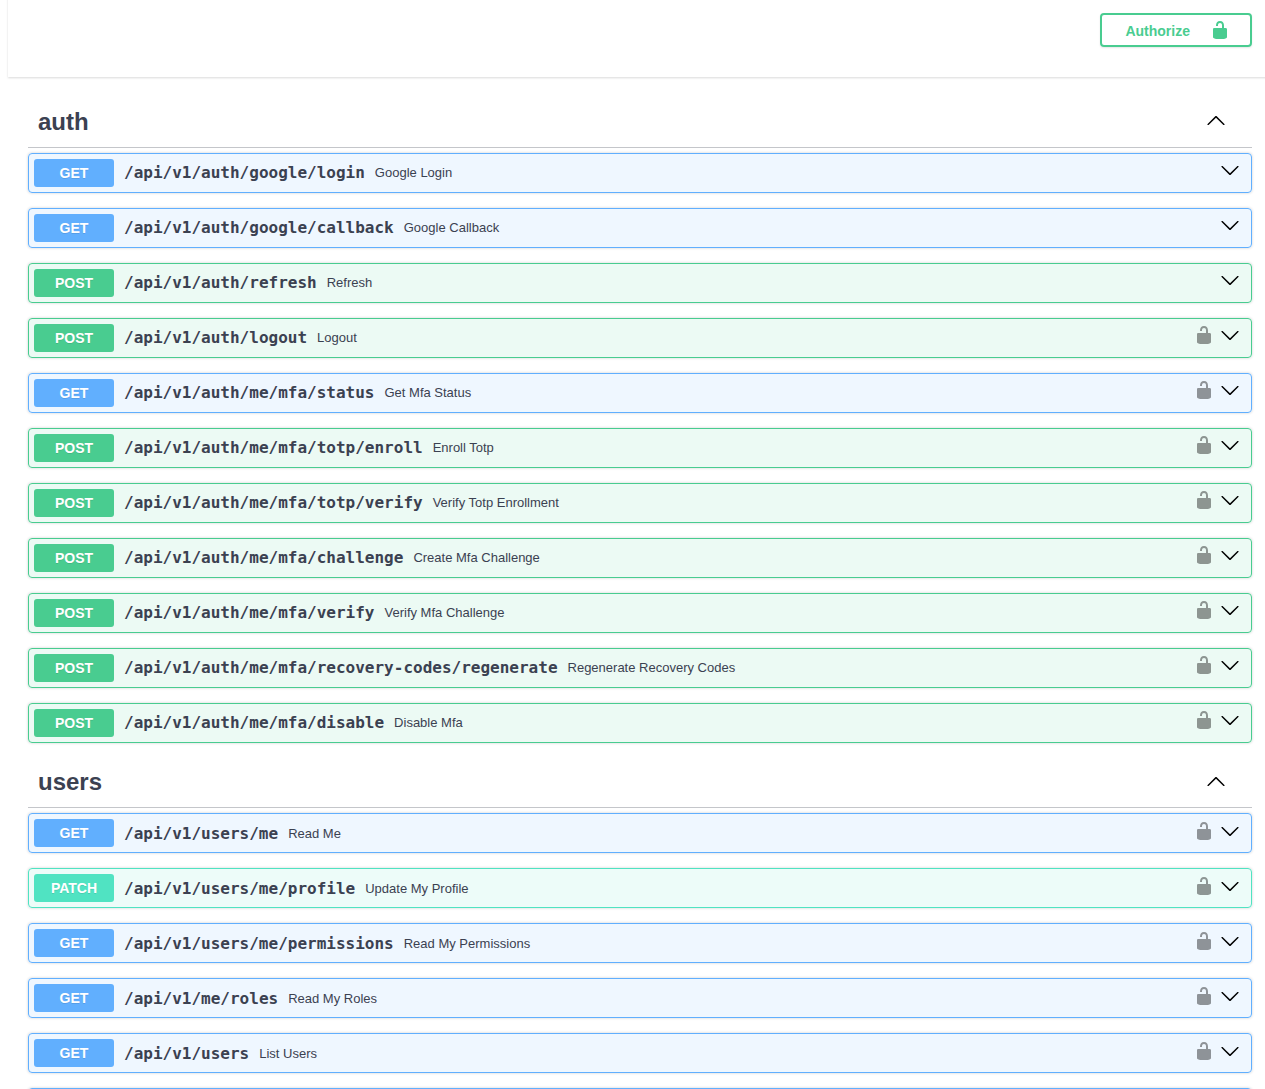
\includegraphics[width=\textwidth,height=0.82\textheight,keepaspectratio]{graphics/swagger/01_auth.png}
    \caption{Swagger UI --- Authentication endpoints. Google OAuth login/callback, refresh, logout, and TOTP-based MFA enrolment, challenge, verify, recovery-code regeneration, and disable.}
    \label{fig:swagger_01_auth}
\end{figure}

\begin{figure}[H]
    \centering
    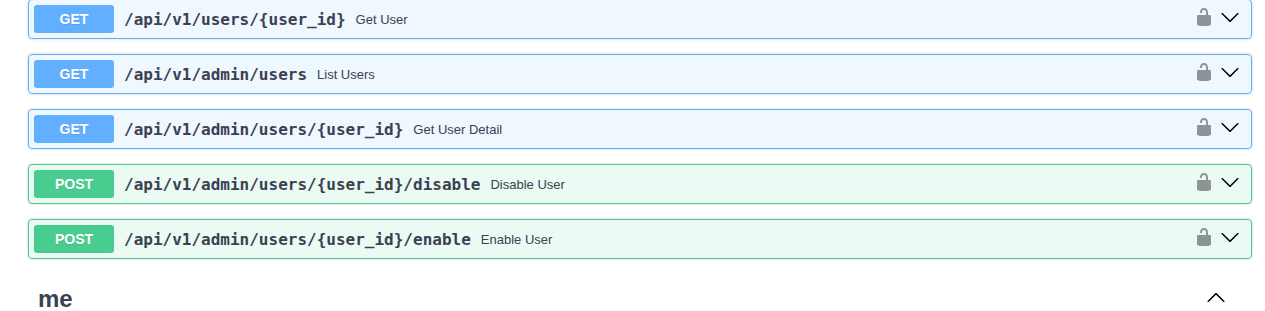
\includegraphics[width=\textwidth,height=0.82\textheight,keepaspectratio]{graphics/swagger/02_mfa.png}
    \caption{Swagger UI --- MFA management. Self-service multi-factor authentication endpoints under \texttt{/auth/me/mfa}.}
    \label{fig:swagger_02_mfa}
\end{figure}

\begin{figure}[H]
    \centering
    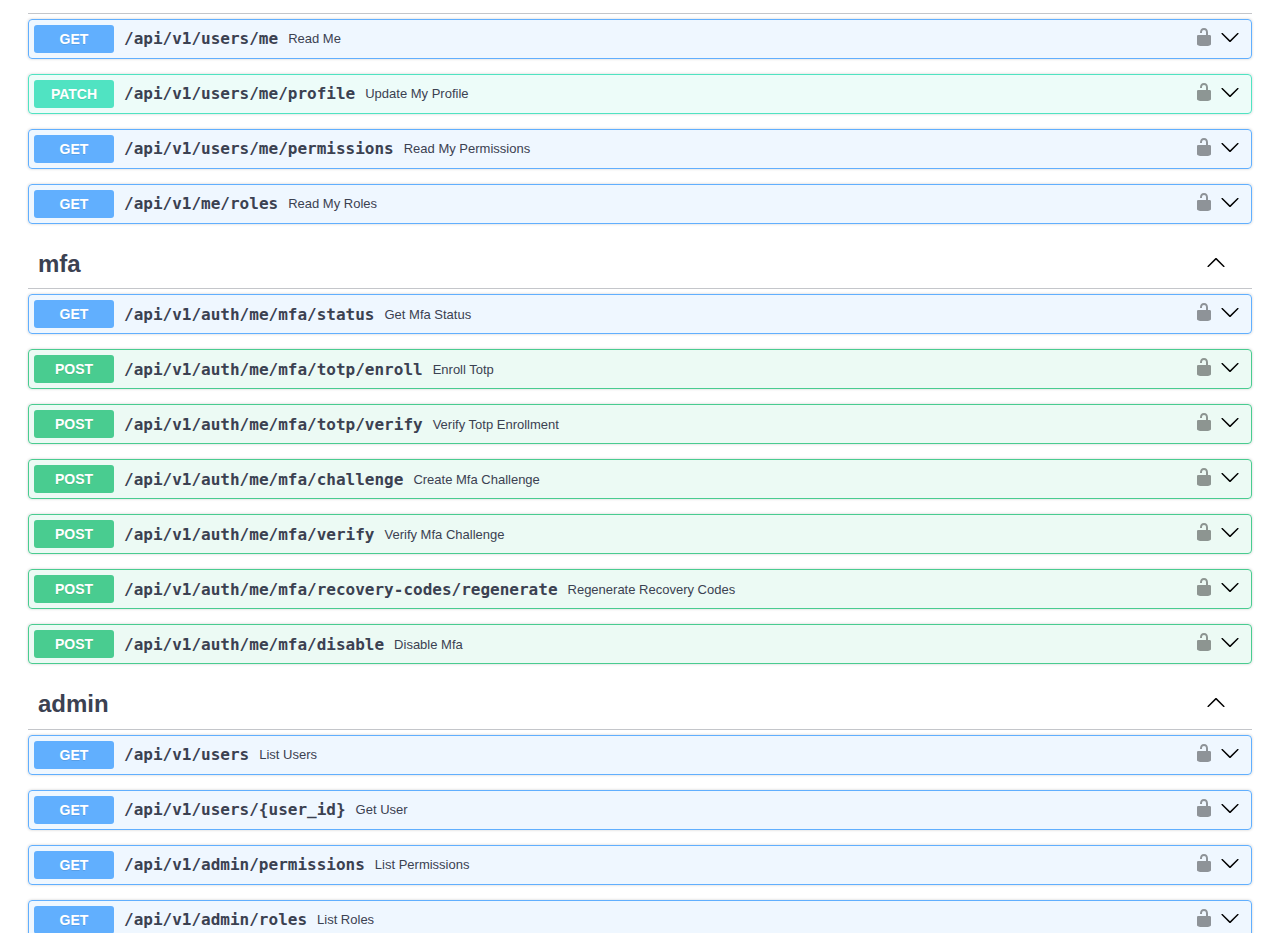
\includegraphics[width=\textwidth,height=0.82\textheight,keepaspectratio]{graphics/swagger/03a_admin_part1.png}
    \caption{Swagger UI --- Administration --- part 1. First half of the administrative endpoint surface (user disable/enable, audit subset).}
    \label{fig:swagger_03a_admin_part1}
\end{figure}

\begin{figure}[H]
    \centering
    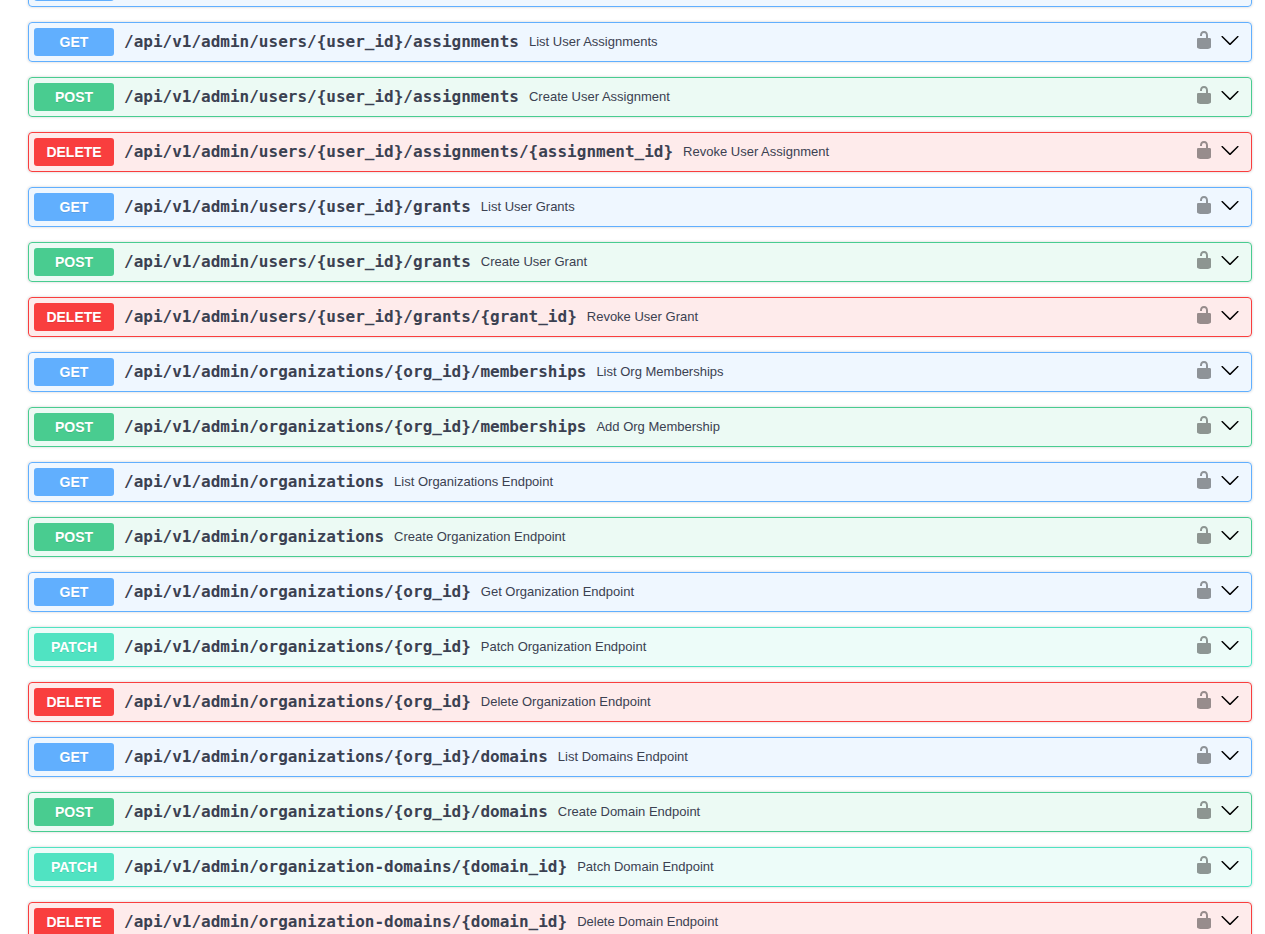
\includegraphics[width=\textwidth,height=0.82\textheight,keepaspectratio]{graphics/swagger/03b_admin_part2.png}
    \caption{Swagger UI --- Administration --- part 2. Remaining administrative endpoints (continued from previous figure).}
    \label{fig:swagger_03b_admin_part2}
\end{figure}

\begin{figure}[H]
    \centering
    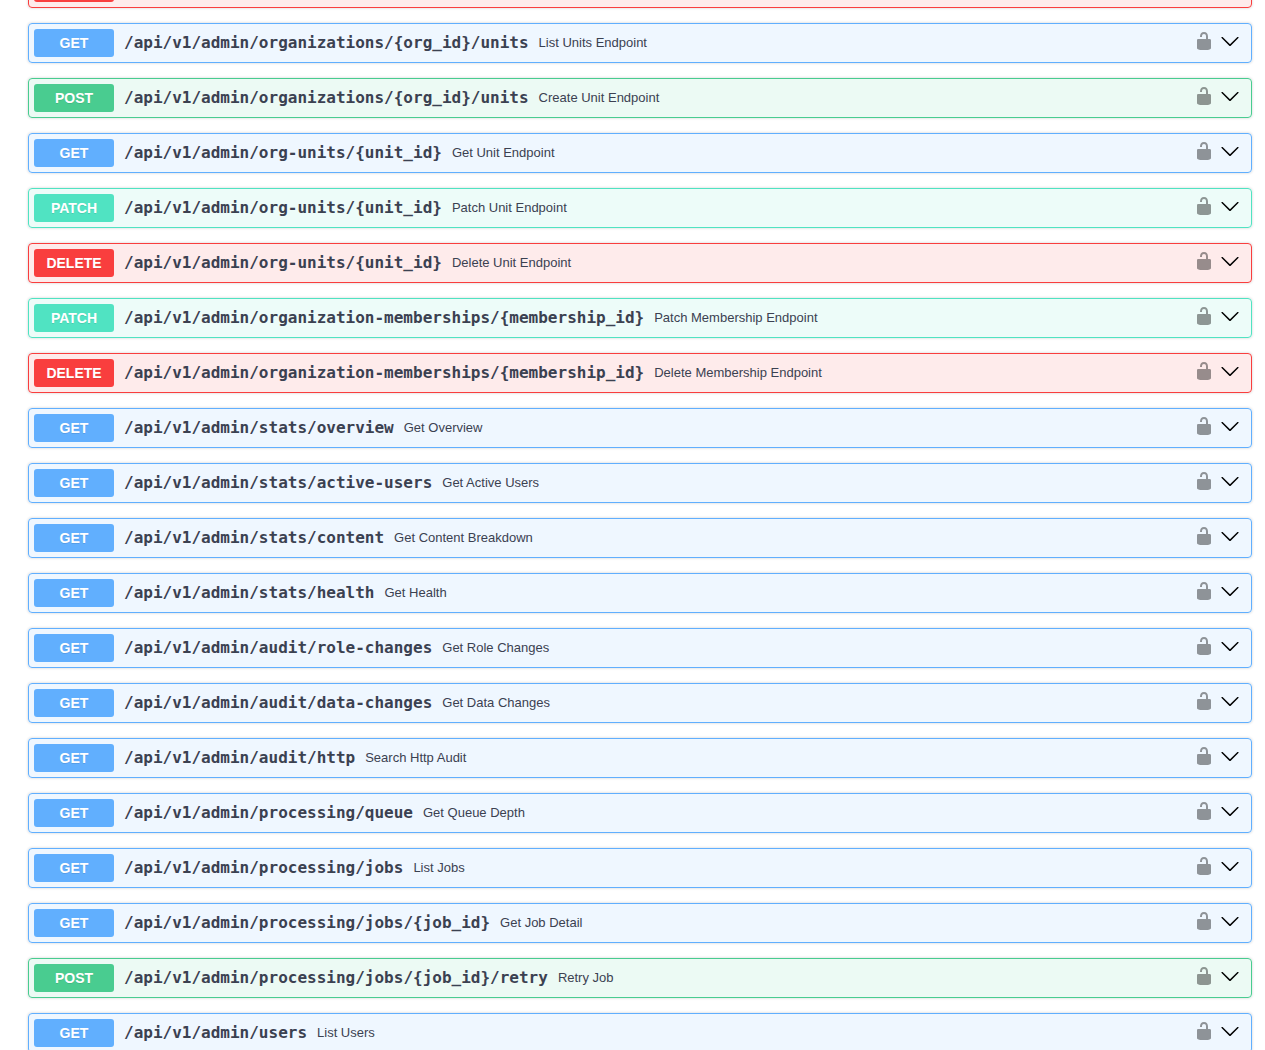
\includegraphics[width=\textwidth,height=0.82\textheight,keepaspectratio]{graphics/swagger/04_access_control.png}
    \caption{Swagger UI --- Access control \& roles. Role assignments, permission grants, organisation-scoped role queries.}
    \label{fig:swagger_04_access_control}
\end{figure}

\begin{figure}[H]
    \centering
    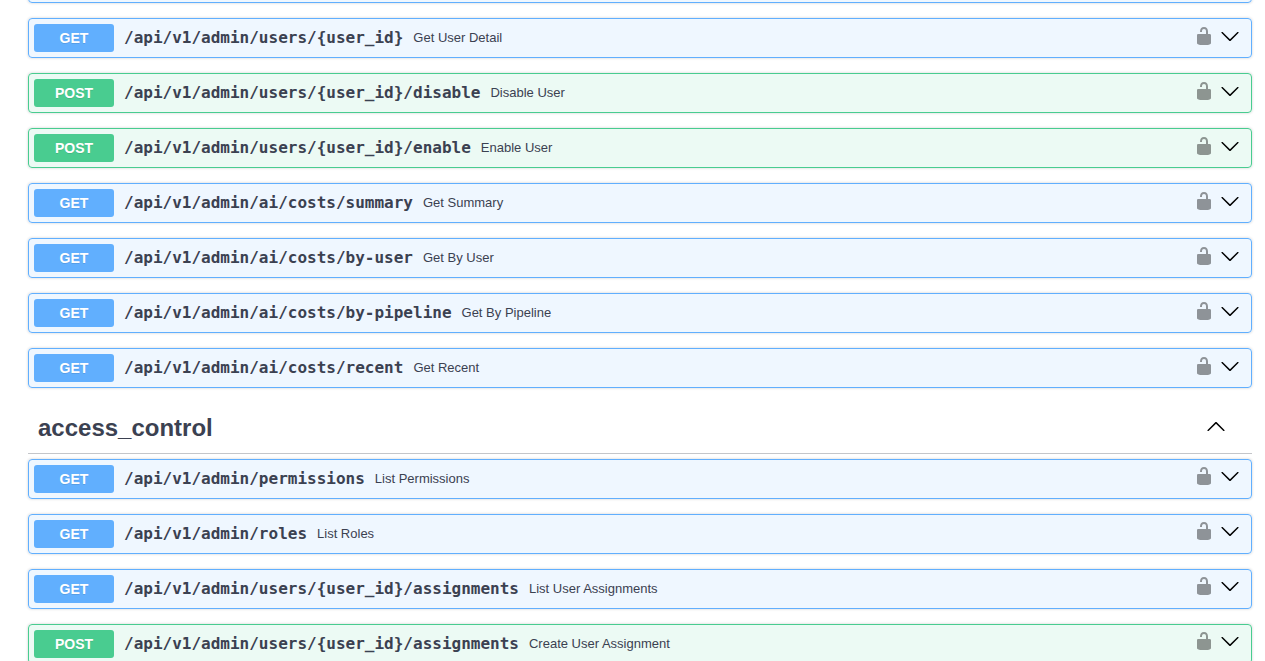
\includegraphics[width=\textwidth,height=0.82\textheight,keepaspectratio]{graphics/swagger/05_organizations.png}
    \caption{Swagger UI --- Organisations. Organisational unit CRUD, hierarchy walk, member listing.}
    \label{fig:swagger_05_organizations}
\end{figure}

\begin{figure}[H]
    \centering
    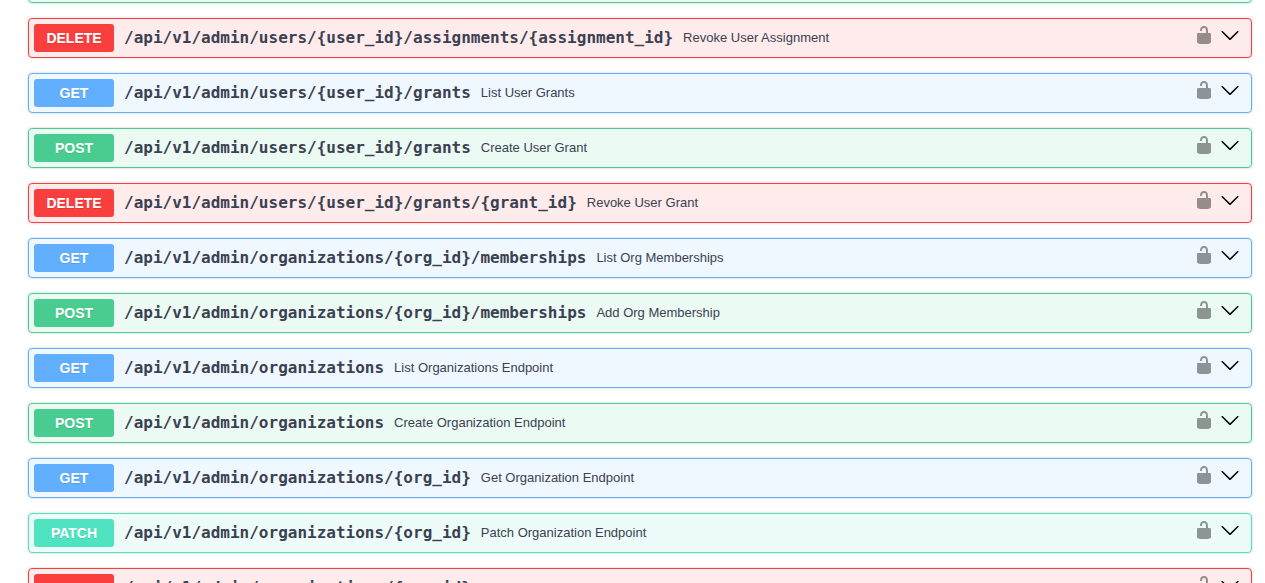
\includegraphics[width=\textwidth,height=0.82\textheight,keepaspectratio]{graphics/swagger/06_courses_learner.png}
    \caption{Swagger UI --- Courses --- learner. Published-course catalogue, enrolled-course lookup, and lesson tree for the calling student.}
    \label{fig:swagger_06_courses_learner}
\end{figure}

\begin{figure}[H]
    \centering
    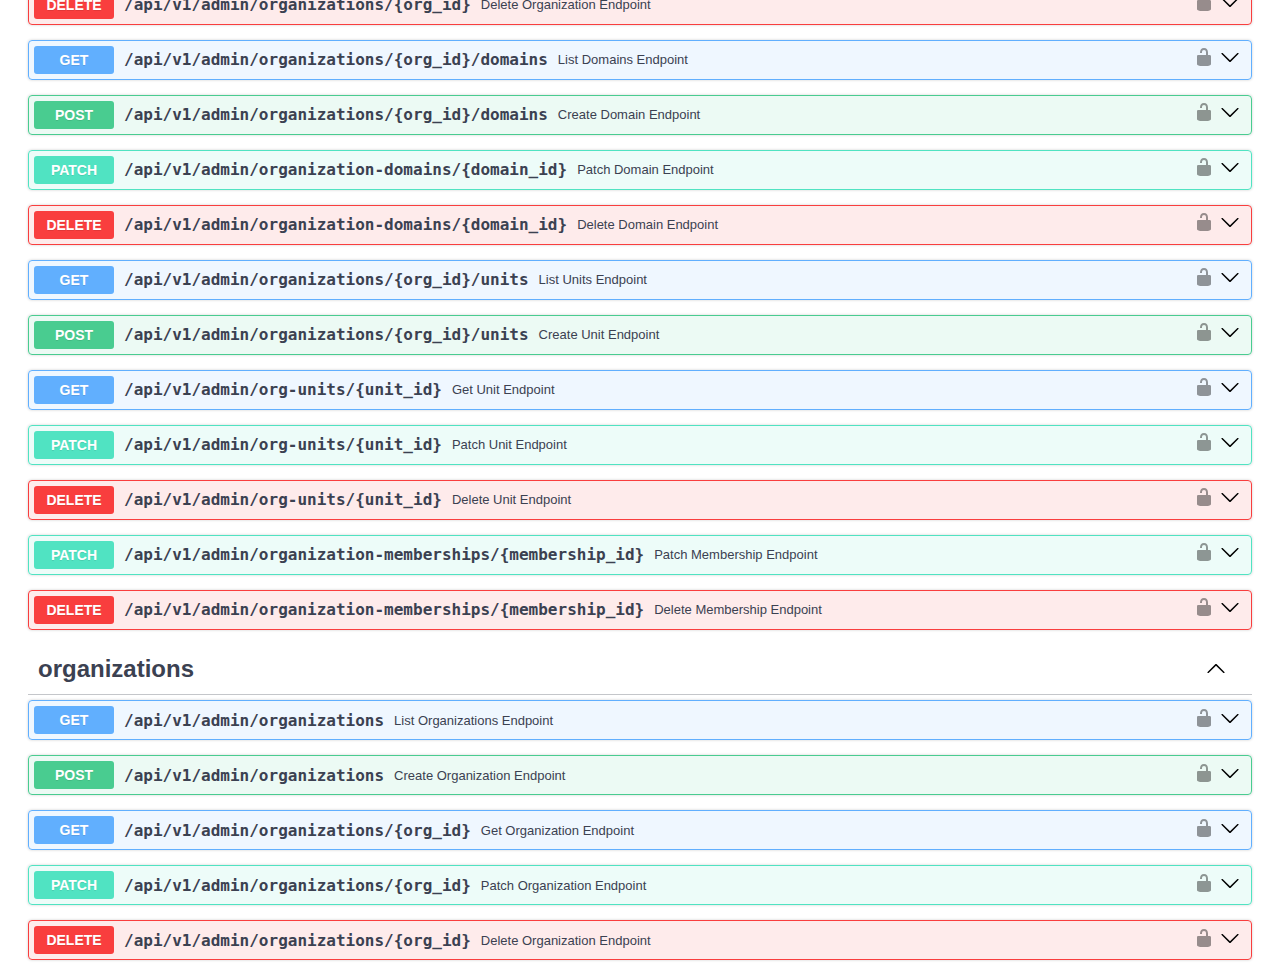
\includegraphics[width=\textwidth,height=0.82\textheight,keepaspectratio]{graphics/swagger/07_courses_authoring.png}
    \caption{Swagger UI --- Courses --- authoring. Instructor course creation, module/lesson editing, publish/archive lifecycle, roster, prerequisites, item reordering.}
    \label{fig:swagger_07_courses_authoring}
\end{figure}

\begin{figure}[H]
    \centering
    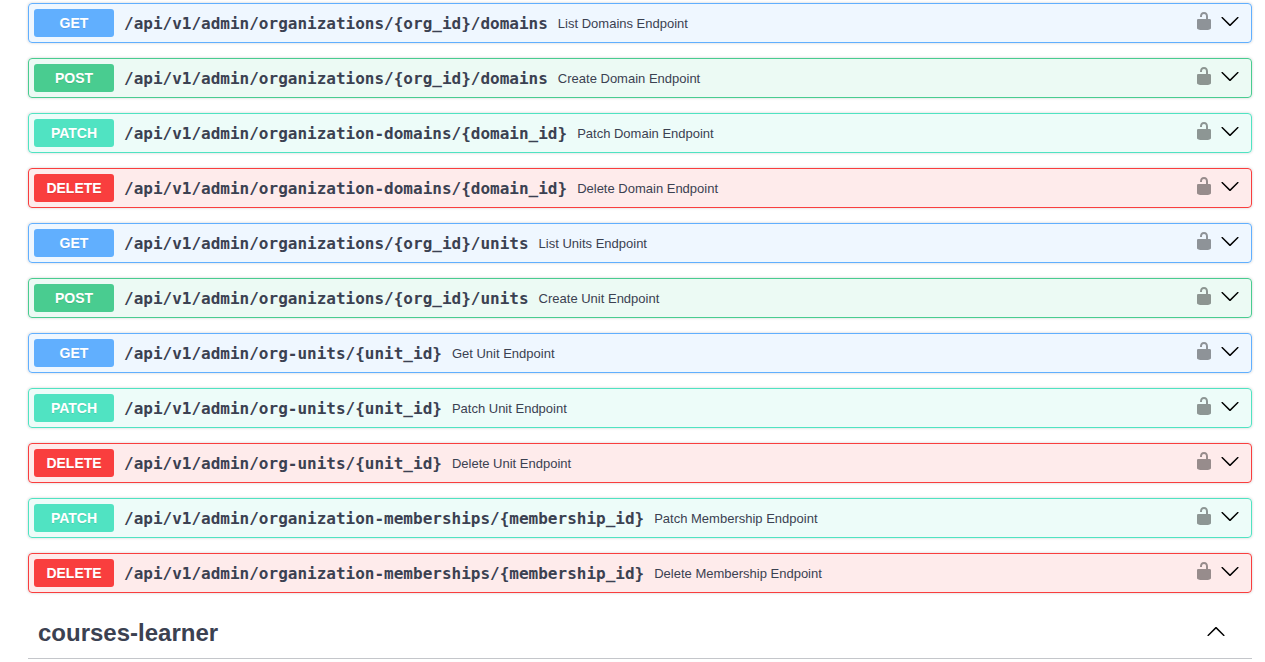
\includegraphics[width=\textwidth,height=0.82\textheight,keepaspectratio]{graphics/swagger/08_courses_admin.png}
    \caption{Swagger UI --- Courses --- department \& administration. Department-scoped course assignment to teachers, cross-organisation course listing, soft-delete restoration, and audit views.}
    \label{fig:swagger_08_courses_admin}
\end{figure}

\begin{figure}[H]
    \centering
    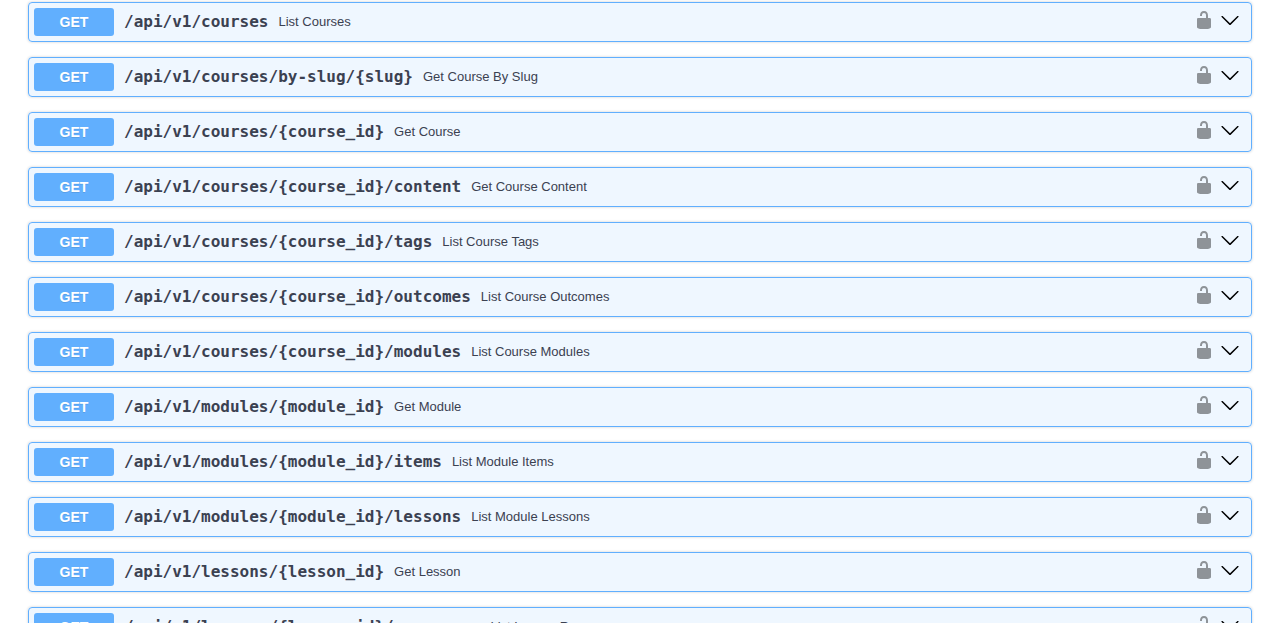
\includegraphics[width=\textwidth,height=0.82\textheight,keepaspectratio]{graphics/swagger/09_materials.png}
    \caption{Swagger UI --- Materials. Two-phase upload protocol (presigned init / multipart parts / complete), processing summaries, learner-facing presigned streaming URLs.}
    \label{fig:swagger_09_materials}
\end{figure}

\begin{figure}[H]
    \centering
    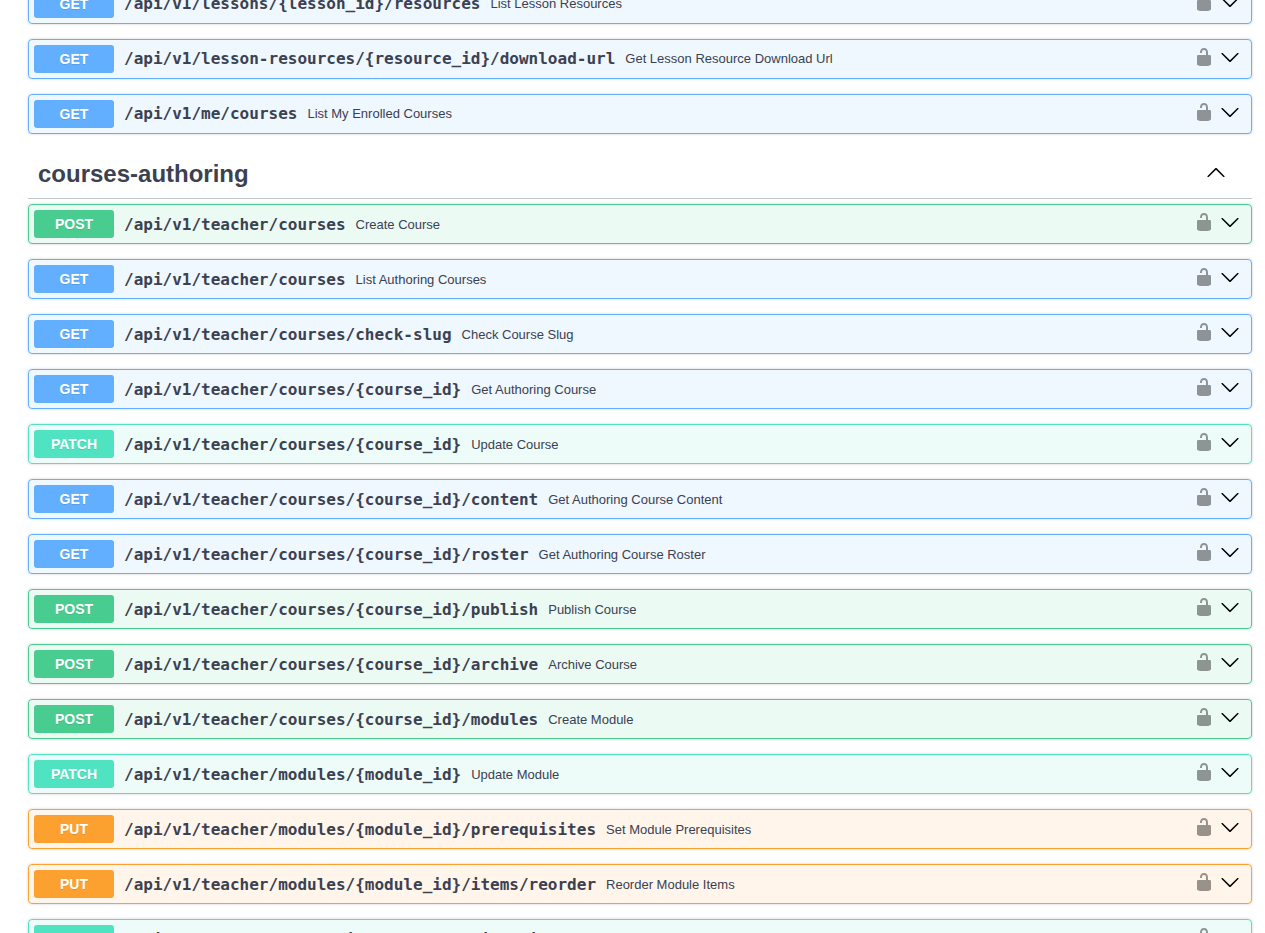
\includegraphics[width=\textwidth,height=0.82\textheight,keepaspectratio]{graphics/swagger/10_quizzes.png}
    \caption{Swagger UI --- Quizzes. Authoring (draft/generate/review/publish) and learner (start attempt, submit, results) endpoints; AI generation through \texttt{generation-runs/\{run\_id\}} polling.}
    \label{fig:swagger_10_quizzes}
\end{figure}

\begin{figure}[H]
    \centering
    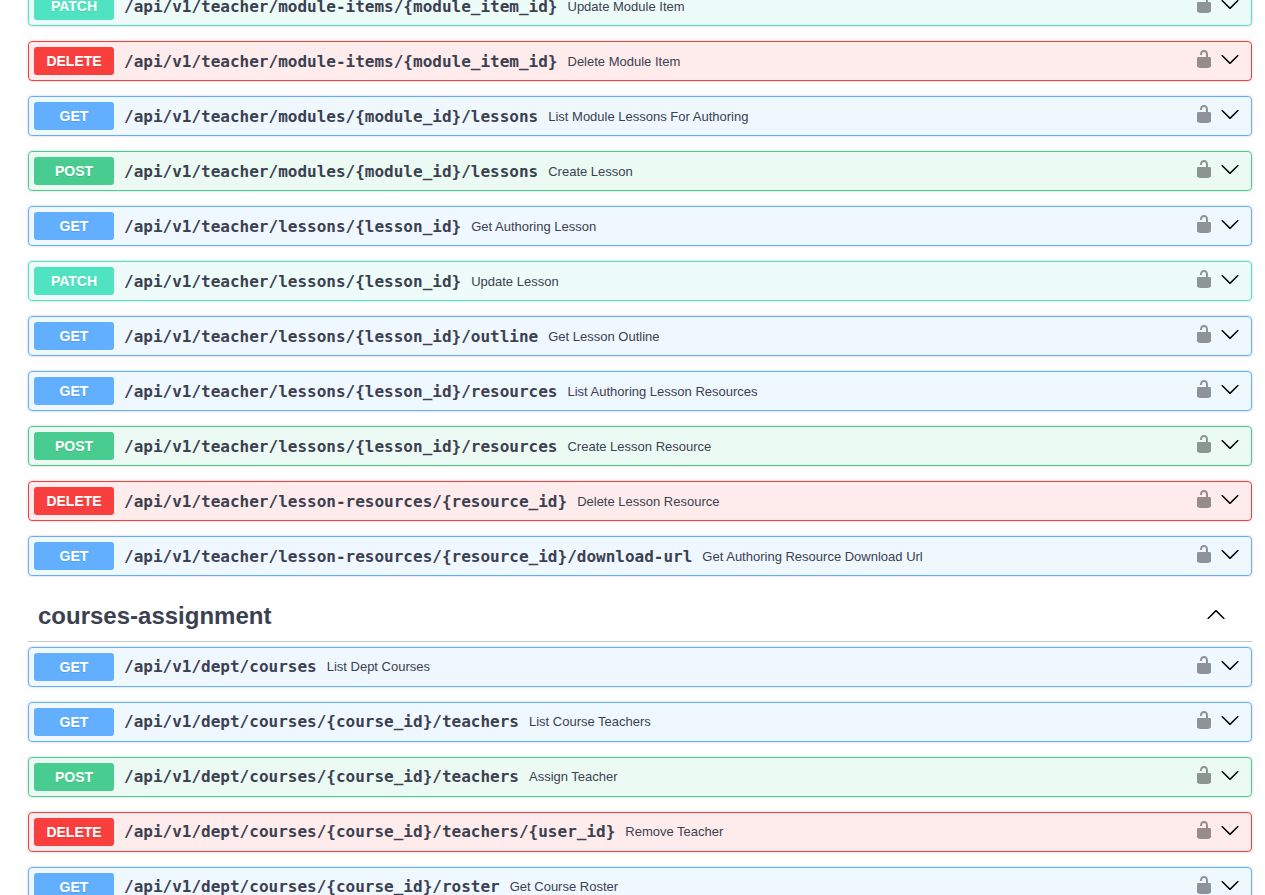
\includegraphics[width=\textwidth,height=0.82\textheight,keepaspectratio]{graphics/swagger/11_interviews.png}
    \caption{Swagger UI --- Interviews. Mock-interview authoring (slots, question banks, regeneration) and learner endpoints (start/submit/feedback).}
    \label{fig:swagger_11_interviews}
\end{figure}

\begin{figure}[H]
    \centering
    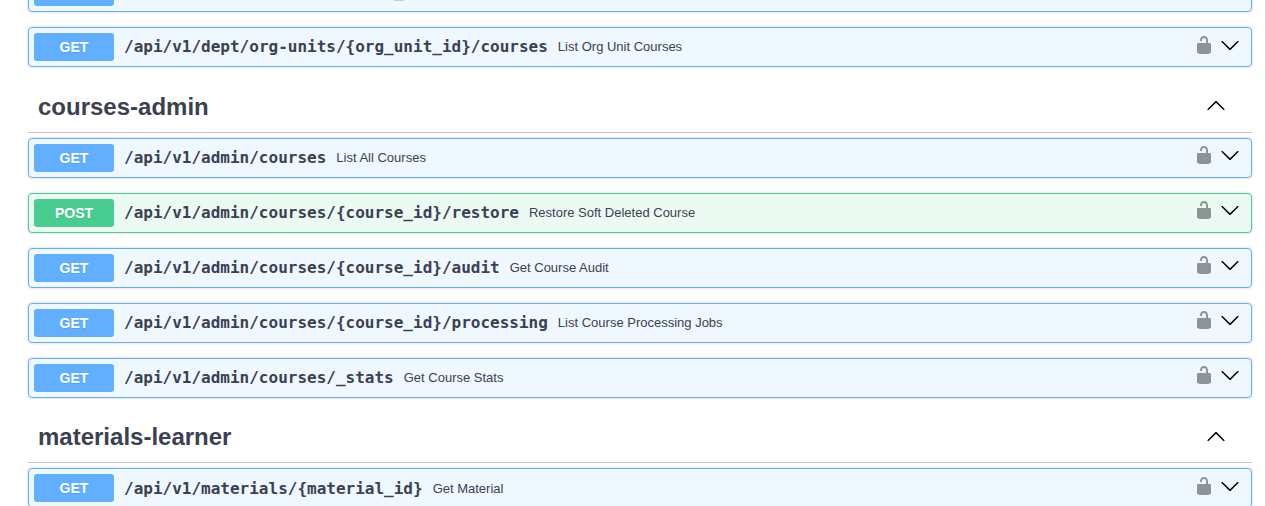
\includegraphics[width=\textwidth,height=0.82\textheight,keepaspectratio]{graphics/swagger/12_enrollments.png}
    \caption{Swagger UI --- Enrollments. Learner self-enrolment and department-assigned enrolment management.}
    \label{fig:swagger_12_enrollments}
\end{figure}

\begin{figure}[H]
    \centering
    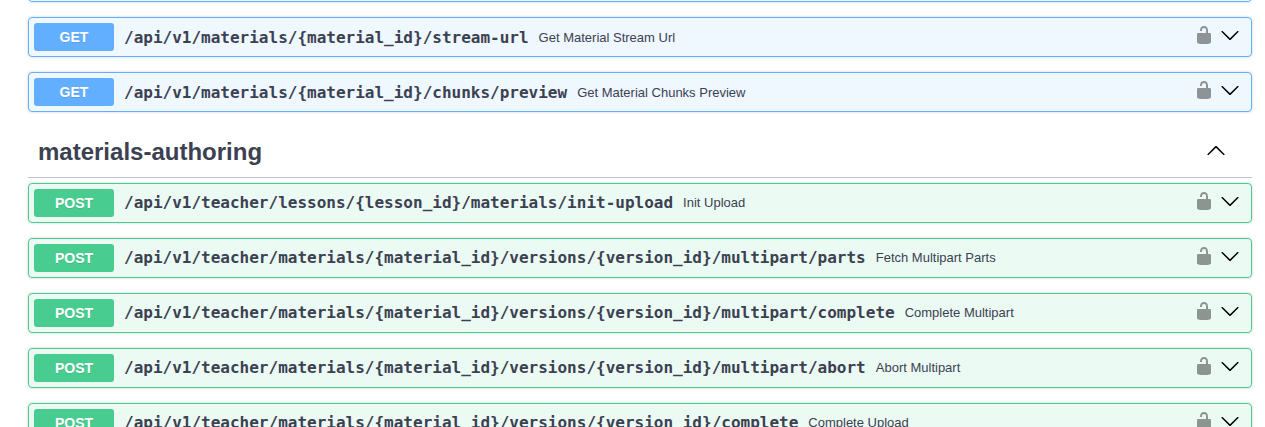
\includegraphics[width=\textwidth,height=0.82\textheight,keepaspectratio]{graphics/swagger/13_progress.png}
    \caption{Swagger UI --- Progress. Learner progress tracking and instructor progress dashboards.}
    \label{fig:swagger_13_progress}
\end{figure}

\begin{figure}[H]
    \centering
    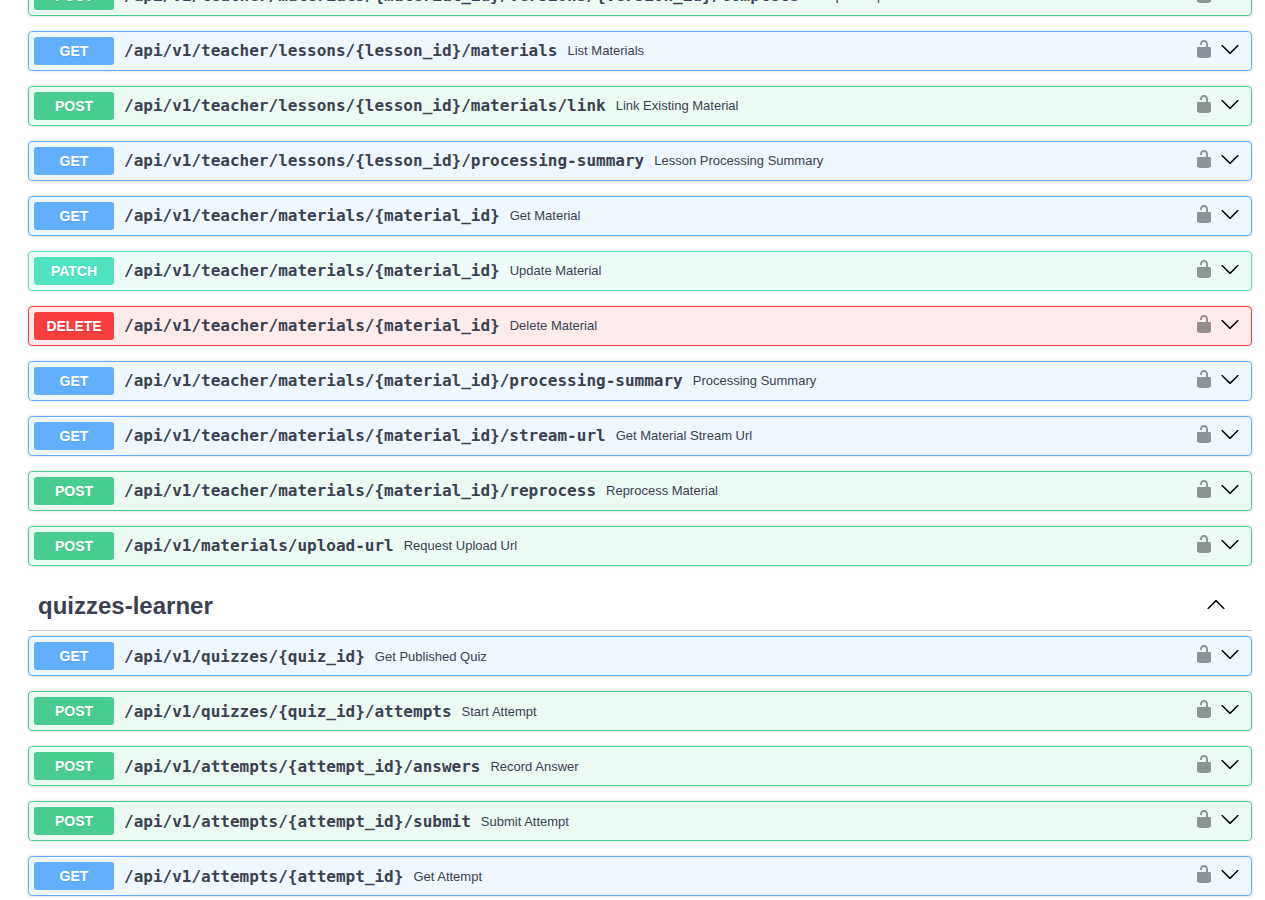
\includegraphics[width=\textwidth,height=0.82\textheight,keepaspectratio]{graphics/swagger/14_career_paths.png}
    \caption{Swagger UI --- Career paths. Published career-path catalogue (learner) and authoring routes (instructor/admin).}
    \label{fig:swagger_14_career_paths}
\end{figure}

\begin{figure}[H]
    \centering
    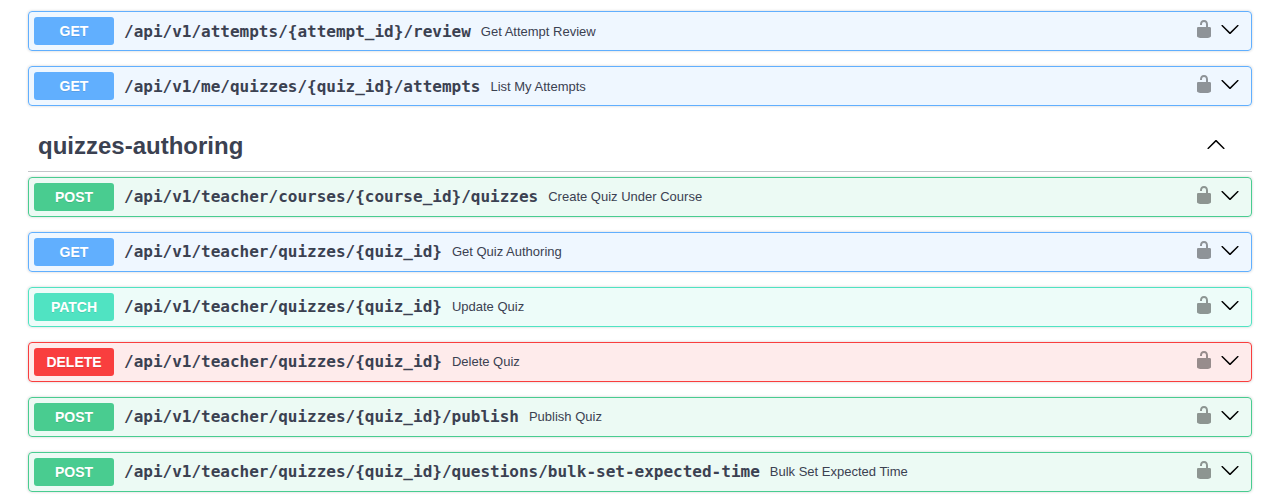
\includegraphics[width=\textwidth,height=0.82\textheight,keepaspectratio]{graphics/swagger/15_notifications.png}
    \caption{Swagger UI --- Notifications \& stats. Learner notification inbox (cursor-paginated by \texttt{created\_at}) and admin platform-wide statistics.}
    \label{fig:swagger_15_notifications}
\end{figure}

\begin{figure}[H]
    \centering
    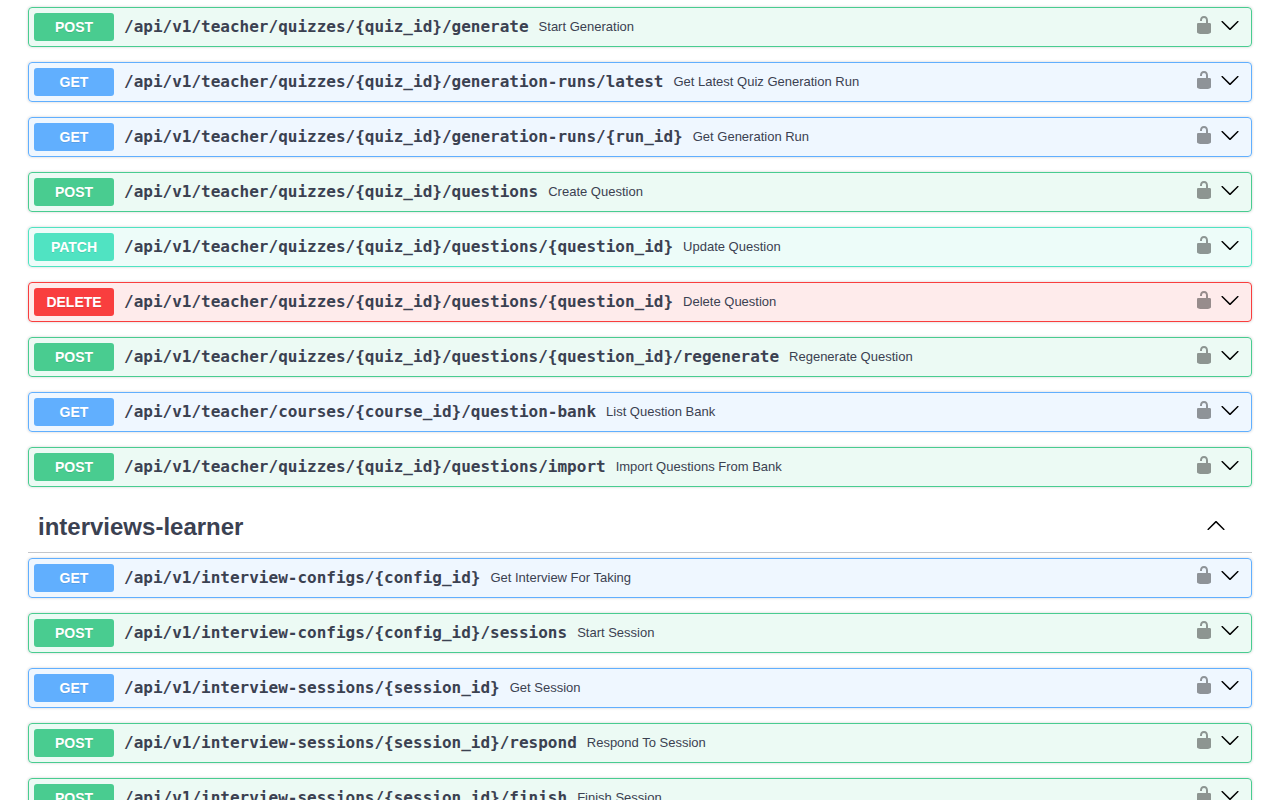
\includegraphics[width=\textwidth,height=0.82\textheight,keepaspectratio]{graphics/swagger/16_audit_processing.png}
    \caption{Swagger UI --- Audit \& processing. Cross-feature audit log queries and AI-processing run inspection (admin).}
    \label{fig:swagger_16_audit_processing}
\end{figure}

\begin{figure}[H]
    \centering
    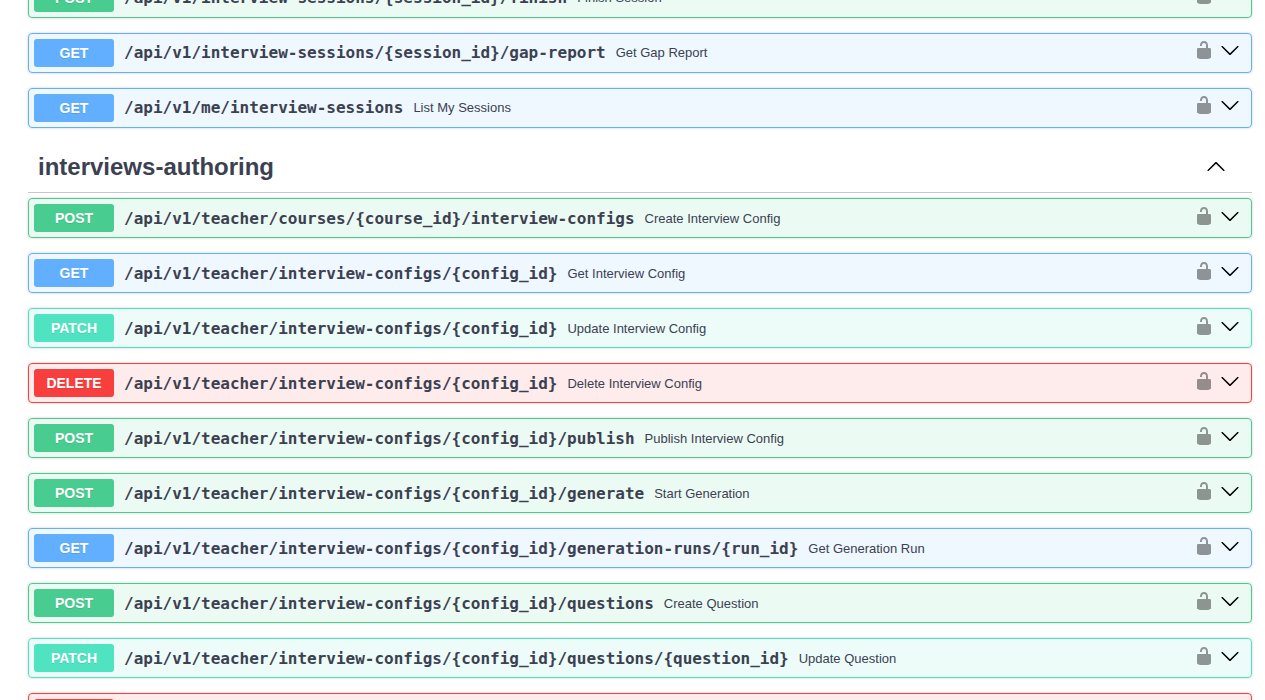
\includegraphics[width=\textwidth,height=0.82\textheight,keepaspectratio]{graphics/swagger/17_spaced_repetition.png}
    \caption{Swagger UI --- Spaced repetition. Learner card-due queue, review submission, lesson-unlock checks, and instructor analytics.}
    \label{fig:swagger_17_spaced_repetition}
\end{figure}

\begin{figure}[H]
    \centering
    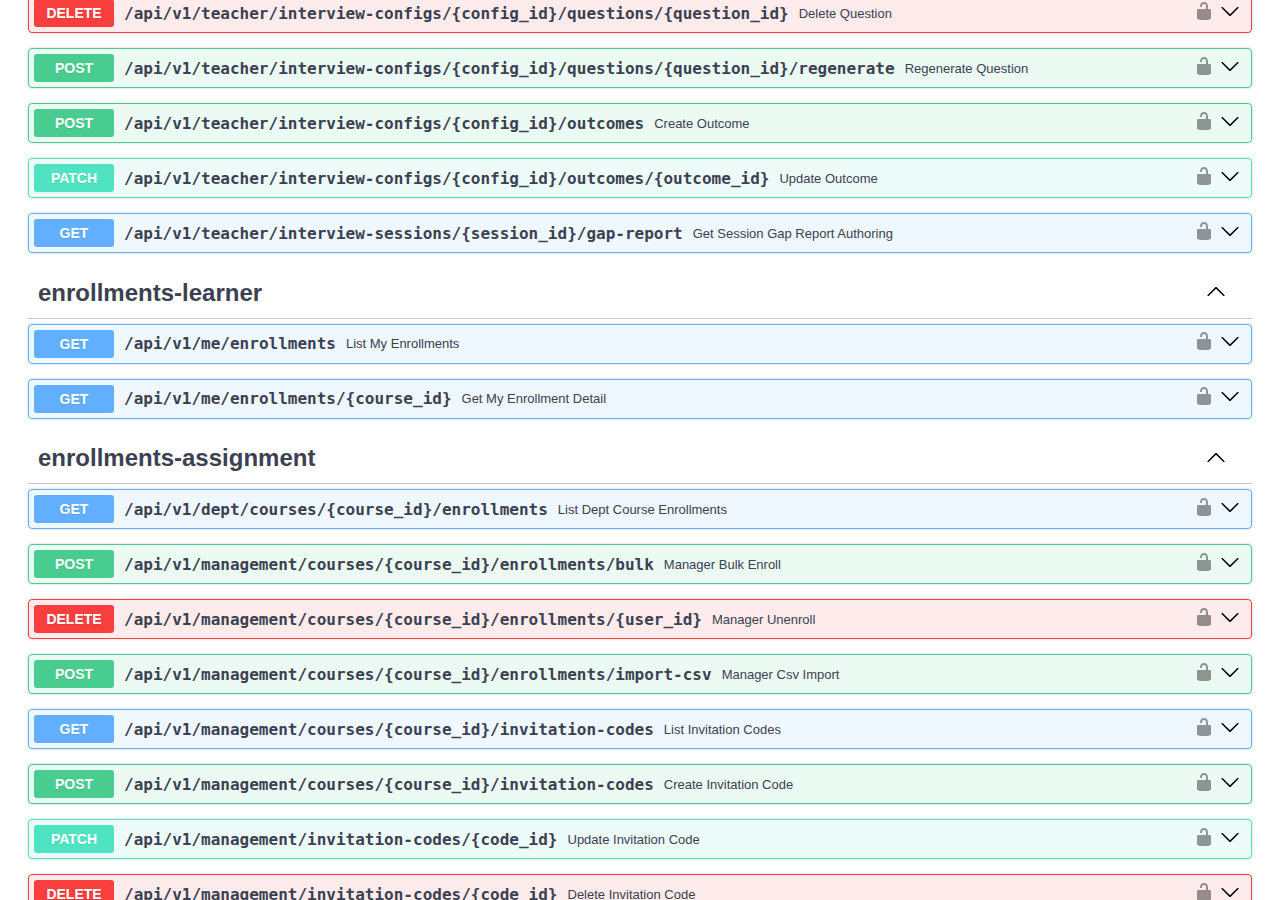
\includegraphics[width=\textwidth,height=0.82\textheight,keepaspectratio]{graphics/swagger/18_ai_costs_health.png}
    \caption{Swagger UI --- AI costs \& health. AI-cost telemetry endpoints and Kubernetes liveness/readiness probes (\texttt{/healthz}, \texttt{/readyz}).}
    \label{fig:swagger_18_ai_costs_health}
\end{figure}

\begin{figure}[H]
    \centering
    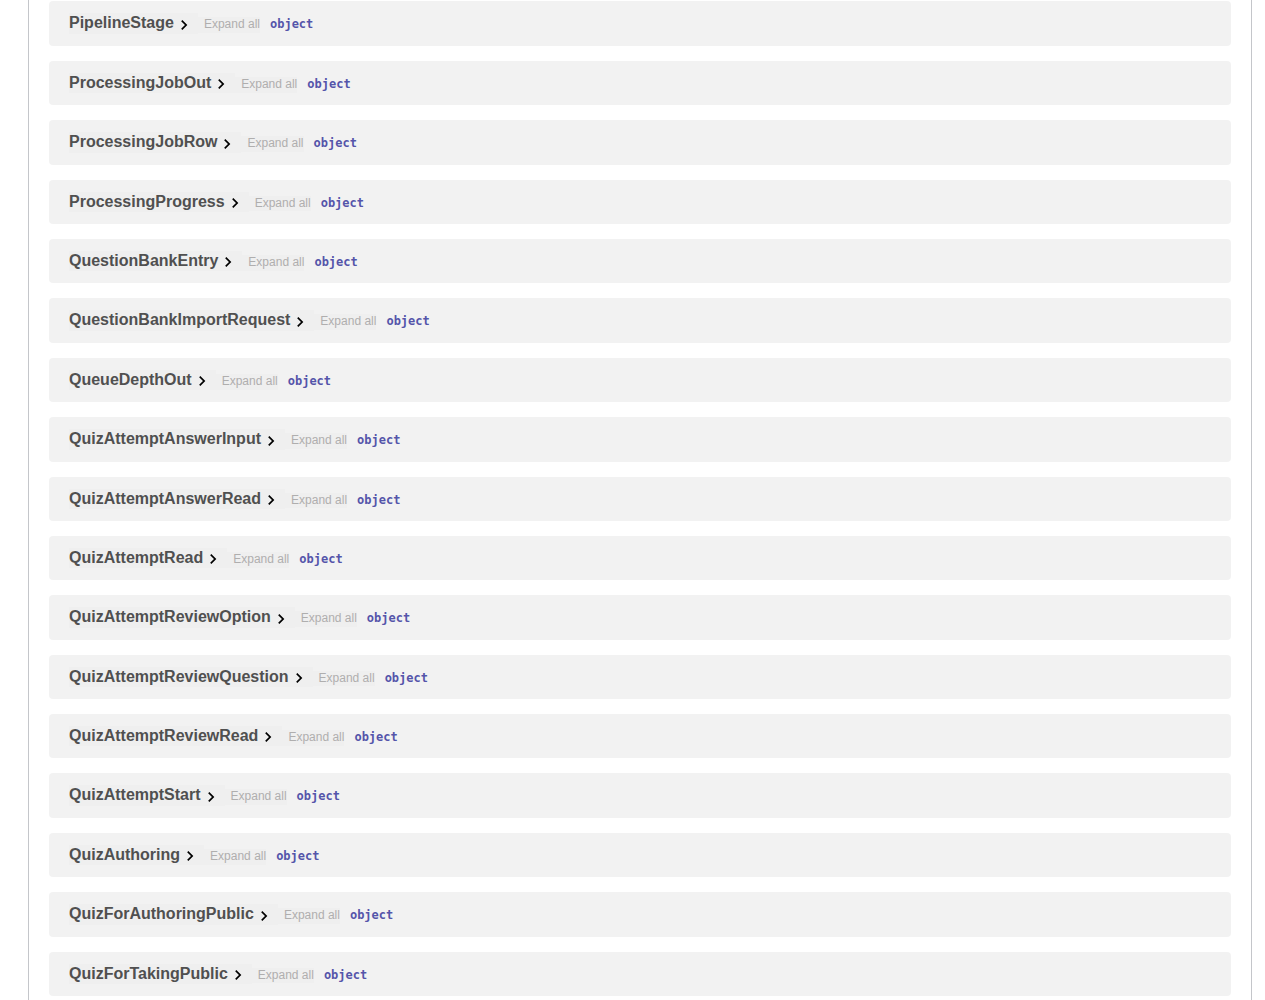
\includegraphics[width=\textwidth,height=0.82\textheight,keepaspectratio]{graphics/swagger/19a_models_part1.png}
    \caption{Swagger UI --- Schemas --- part 1. Pydantic v2 schemas exposed in OpenAPI \texttt{components.schemas} (first third of 223 schemas).}
    \label{fig:swagger_19a_models_part1}
\end{figure}

\begin{figure}[H]
    \centering
    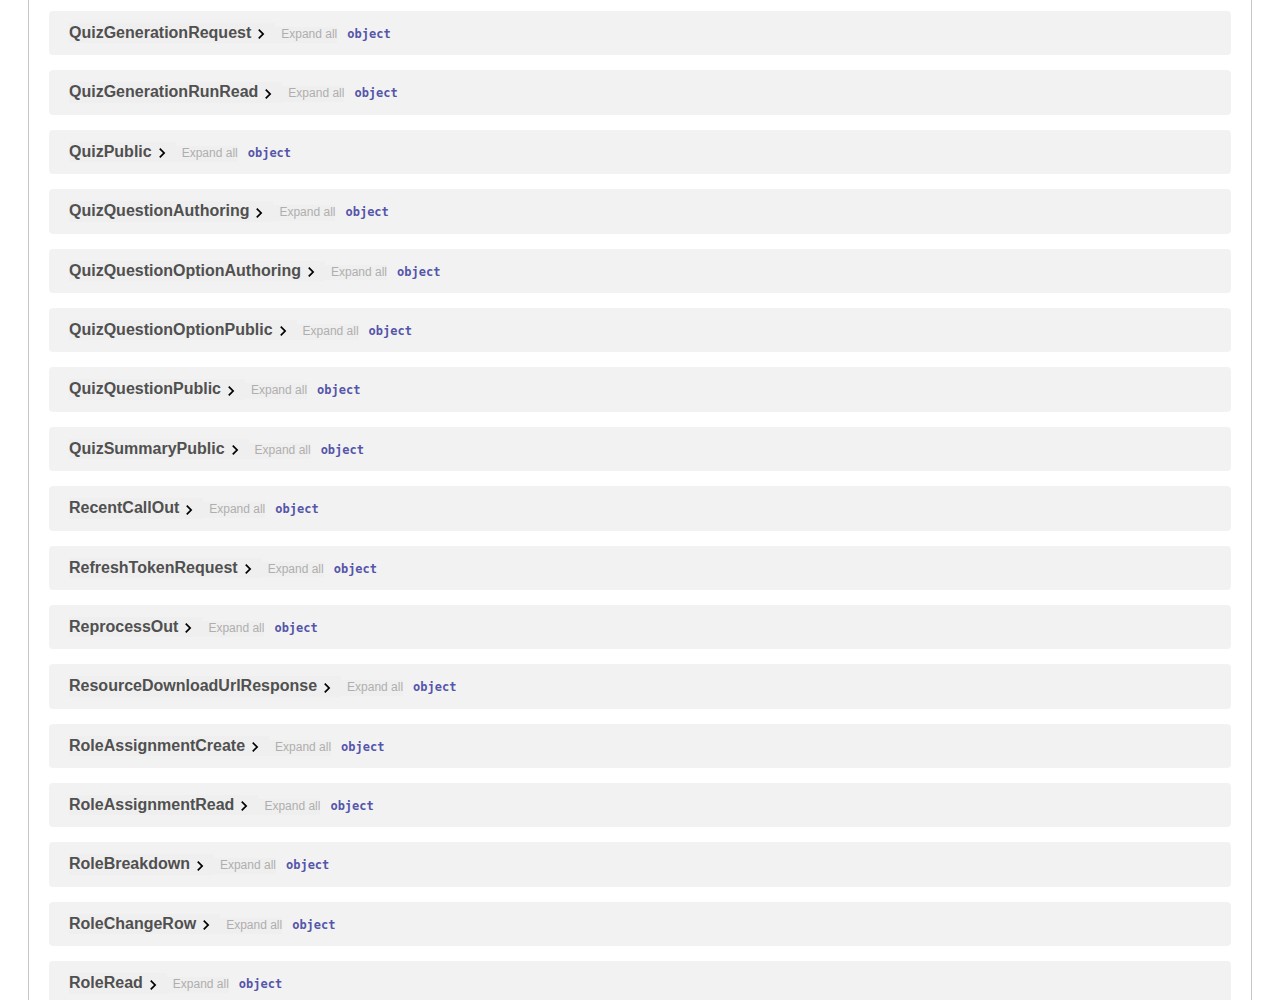
\includegraphics[width=\textwidth,height=0.82\textheight,keepaspectratio]{graphics/swagger/19b_models_part2.png}
    \caption{Swagger UI --- Schemas --- part 2. Pydantic v2 schemas (continued).}
    \label{fig:swagger_19b_models_part2}
\end{figure}

\begin{figure}[H]
    \centering
    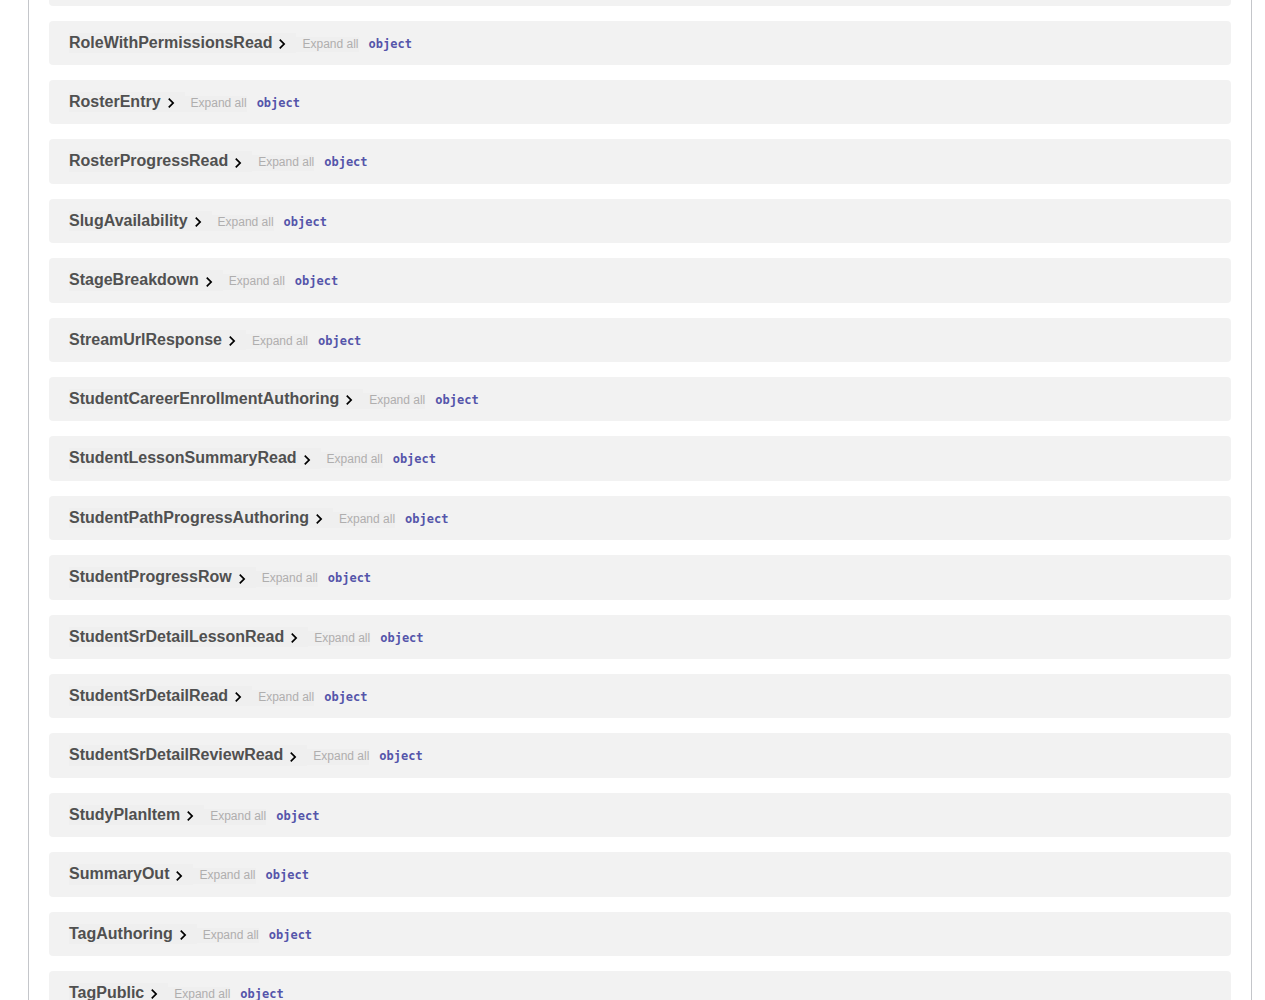
\includegraphics[width=\textwidth,height=0.82\textheight,keepaspectratio]{graphics/swagger/19c_models_part3.png}
    \caption{Swagger UI --- Schemas --- part 3. Pydantic v2 schemas (final third).}
    \label{fig:swagger_19c_models_part3}
\end{figure}
